
\documentclass[../main.tex]{subfiles}
\begin{document}
\newcommand{\jin}[1]{j^{\textrm{in}}(#1)}
\newcommand{\jout}[1]{j^{\textrm{out}}(#1)}

\chapter{Lucky drops grow bigger: but luckier drops get less lucky}\label{lck-drp}

% \textit{Rajarshi\orcidlink{0009-0009-1747-3916}, Rama Govindarajan. International Centre for Theoretical Sciences, Bengaluru.}

\begin{summary}
\begin{itemize}
    \item In $2$D: luckier lucky droplets are at a disadvantage.
    \item In $2$D: Particles starting out in high vortical regions grow faster.
    \item In $2$D: Intermediate stage growth rate is larger than a random walk.
    \item In $3$D: Disadvantage / advantage of larger lucky droplets. \\
        Growth rate v crossing the threshold.
    \item In $3$D: how does gravity change the equation?
\end{itemize}
\end{summary}

\section{Introduction}

Knowing which clouds will rain, and correctly calculating the cloud cover over the Earth, is crucial in predicting local weather and global climate. This requires us to quantitatively understand how water droplets of a few $\mu$m grow to raindrops of a few mm. However, a long-standing unanswered question is how cloud droplets of sizes 10 $\mu$m grow to sizes of 50 $\mu$m in a few hours. For droplets of these sizes, neither collisions-condensation due to Brownian motion, nor collisions while settling under gravity are enough for the required growth in time to rain  \cite{grabowski2013}. Three decades ago, scientists suggested that turbulent advection of these droplets may cause them to dash against each other. They collide, coalesce, and thereby grow. Once particles attain large enough sizes ($>50 \mu$m), they settle faster under gravity and encounter more droplets on their way, growing till they fall as raindrops.

Unfortunately, the debate whether the turbulent flow of the atmosphere is enough for the timely growth of $10-50\mu$m droplets is still unsettled. Two decades ago, \citet{falkovich2002} argued that finitely sized droplets can detach from the flow and collide with each other. This was followed up \cite{shaw2003,wilkinson2006,falkovich2007} and generated significant interest to look at particle collisions in turbulence from both Lagrangian and Eulerian frameworks.

On the experimental side of things, \citet{toschi2009} and \citet{bewley2013} studied particle collision-coalescence in a lab with a turbulence chamber. They observed sling effects predicted by \cite{falkovich2002,shaw2003,wilkinson2006}. The remaining goal of the theorists was to match their theory quantitatively with these experimental findings. However, such efforts using both Lagrangian and Eulerian frameworks have failed due to multiple reasons.

Setting other factors aside, like electrical charges on the cloud droplets, or the effect of their deformed geometry, or their complicated hydrodynamic interactions when they collide, the Eulerian description fails as they have singularities. Closures approximations to avoid these singularities, like the ones used in \citet{kasbaoui2019} do not particularly match Lagrangian particle dynamics. In addition, most Eulerian models used for particles are monodisperse. One needs to use a separate field for every particle size, making it computationally very expensive \cite{li2017}. However, existing analysis of such studies neglects collisions of particles of the same size, requiring even smaller size bins for the particle fields. This line of work requires a good theoretical framework.

Direct numerical simulations of water droplets have so far been the sensible option to extract physics from this problem. However, even with billions of particles suspended in turbulent flow resolved with tens of billions of grid points, \cite{bec2016} could only study cases where the mass of a particle increased by 15 times. Compare that to a particle that grows from $10\mu$m to $50\mu$m. Its mass increases by 125 times, an order of magnitude more than what was captured by \cite{bec2016}. Recently, \cite{batge2026} fit the data from their DNS simulations to extrapolate to cases with higher Reynolds numbers and particle mass sizes. However, their fit also came from small increases in mass.

The more widely used Lagrangian modelling of the cloud droplets is the `super-droplet' method of \citet{shima2009} and its various versions. Here, swarms or super-drops of the cloud particles are evolved as if they were a single particle. Every particle in a particular swarm has the same size. The number of particles in a swarm can change when different swarms collide with each other. The different super-droplet methods vary in their collision schemes \cite{li2017}. Although this is an oversimplified model, it performs surprisingly well for cases with condensation growth \cite{li2017, grabowski2021}, and convergence studies for non-precipitating clouds \cite{sato2017}. Accordingly, most of the studies using the super-droplet method focus either on the condensation growth or on the gravitational settling, and not on the turbulence-accelerated growth. Such crude approximations for poly-disperse distribution of particles are expected to fail in a turbulent flow. However, a conclusive study on the effect of turbulence on collision-coalescence of cloud droplets using the super-droplet method is yet to be done \cite{liu2023}.

Current modelling of rain in the atmosphere is even cruder. A mixing ratio quantifying water-vapor mass to dry air mass is advected as tracers, with evaporation from the sea and updraft acting as its sources, and precipitation as its sink \cite{lapeyre2004,brown2023}. Precipitation or rain is triggered when the mixing ratio exceeds a threshold of thermodynamic supersaturation, and the former is relaxed to the threshold value. However, supersaturation is not the only factor that would trigger rain. A supersaturated volume of fluid will only form rain if there are enough large droplets that sediment fast enough to collect other droplets. In other words, in addition to the cloud parcel being supersaturated, precipitation hinges on whether the size distribution of the droplets has a fat enough tail. The latter fact is either poorly captured or not captured at all in current models. This is where a first-principle derivation of the hydrodynamic equations of polydisperse particles comes to play.


A recent school of thought has been the following: once, particles of large enough sizes are created from the sea of small particles, they follow significantly different trajectories from their smaller counterpart, and turbulent air will make them collide more with more smaller particles, making them grow even faster. These accidental large particles, termed `lucky drops', are thought to be enough to initiate rain, even when only one in a million particles turn out lucky. \textbf{cite}.

In this work we investigate whether this is true. Confining ourselves to a fixed number mass of lucky drops, we investigate whether which of the following grow faster, fewer luckier drops, or larger less lucky drops? We approximate the complicated system in two ways. First, we assume a mono-disperse point particles that do not collide with each other. Rather they are advected by turbulent flow. We seed the lucky drops with a certain size and neglect collisions between any two lucky particles. Although, here we will try to justify it, we must confess that these approximations are made to make the dynamics simple. The first approximation allows us to write field equations of the small particles, which are accurate and are devoid of singularities. The field equation also makes capturing collision between the lucky droplets and the smaller ones. Instead of checking crossing between billions of particles, we can write down ordinary differential equations for growth rate of individual lucky droplets. And, the complexity of the calculating particle crossing forces us to make the second assumption.

We find a few surprising results. First, we see that for a fixed volume fraction and
\section{Non-dimensional cloud numbers}
The kinematic viscosity of air $\nu = 10^{-5}\mbox{m}^2\cdot\mbox{sec}^{-1}$. Observation suggests that mean dissipation rate in warm clouds can range from $10^{-3}\mbox{m}^2\cdot\mbox{sec}^{-3}$ to $10^{-1}\mbox{m}^2\cdot\mbox{sec}^{-3}$ (see \citet{grabowski2013} \S 2.1). This sets the Kolmogorov timescale $\tau_\eta = \sqrt{\nu/\epsilon}$ to be $0.1$ to $0.01$ sec, respectively. Similarly, the Kolmogorov length scale $\eta = (\nu^3/\epsilon)^{1/4}$ ranges from $1\mbox{mm}$ to $0.3\mbox{mm}$, respectively. Now a $1\mu\mbox{m}$(diameter) cloud droplet $1000$ times heavier than the air will have Stokes numbers ranging from $5\times 10^{-5}$ to $5\times 10^{-4}$, respectively. Warm clouds may have $10^{9}$ water droplets in $1\mbox{m}^3$, making the volume fraction $c_s$ of $1\mu\mbox{m}$ droplets to be $5\times 10^{-10}$  The Stokes number scales quadratically with particle sizes and the volume fraction cubically. Thus, particles of $10\mu\mbox{m}$(diameter) will have Stokes ranging from $5\times 10^{-3}$ to $0.05$ and volume fraction of $5\times 10^{-7}$.

\begin{table}[h]
    \centering
    \renewcommand{\arraystretch}{1.6}
    \begin{tabular}{@{} l @{\hspace{1.3em}} c @{\hspace{1.3em}} c @{\hspace{1.3em}} c @{\hspace{1.3em}} c @{\hspace{1.3em}} c @{}}
        \toprule
        & $\epsilon = 10^{-3}\ \text{m}^2\text{s}^{-3}$
        & $\epsilon = 10^{-2}\ \text{m}^2\text{s}^{-3}$
        & $\epsilon = 10^{-1}\ \text{m}^2\text{s}^{-3}$
        & $c$
        & $\tau_{\mbox{coll}}$\\
        \midrule
        $\eta = (\nu^3/\epsilon)^{1/4}$   & $1\ \text{mm}$   & $0.6\ \text{mm}$  & $0.3\ \text{mm}$  & in $1\ \text{m}^3$ & tracer \\
        $\tau_\eta = \sqrt{\nu/\epsilon}$ & $0.1\ \text{s}$  & $0.03\ \text{s}$  & $0.01\ \text{s}$  & $10^9$ particles & assumption\\
        $Fr= \epsilon^{\frac34}/(g\nu^\frac14)$ & $0.01$  & $0.06 $  & $0.3$  &&\\
        \midrule
        $d = 1\ \mu\text{m}$  & $\mathrm{St} = 5.5\times10^{-5}$ & $\mathrm{St} = 1.7\times10^{-4}$ & $\mathrm{St} = 5.5\times10^{-4}$ & $5\times10^{-10}$ &$318$ s\\
        $d = 2.7\ \mu\text{m}$  & $\mathrm{St} = 3.2\times10^{-4}$ & $\mathrm{St} = 1\times10^{-3}$ & $\mathrm{St} = 3.2\times10^{-3}$ & $7.2\times10^{-9}$ &$44$ s\\
        $d = 5\ \mu\text{m}$  & $\mathrm{St} = 1.4\times10^{-3}$ & $\mathrm{St} = 4.2\times10^{-3}$ & $\mathrm{St} = 0.014$ & $6.3\times10^{-8}$ &$13$ s\\
        $d = 10\ \mu\text{m}$ & $\mathrm{St} = 5.5\times10^{-3}$ & $\mathrm{St} = 0.017$            & $\mathrm{St} = 0.055$           & $5\times10^{-7}$  & $3$ s\\
        \bottomrule
    \end{tabular}
    \caption[Kolmogorov scales and droplet parameters for warm clouds]{Kolmogorov scales and particle parameters for warm clouds ($\nu = 10^{-5}\text{m}^2\text{s}^{-1}, u_{\rm rms} = 1\, \mbox{m s}^{-1}$. Values according to \citet{grabowski2013} \S 2.1).}
    \label{lucky-cloud-vals}
\end{table}

%Now, for $ $1\mu\mbox{m}$ and $10 \mu\mbox{m}$ spherical water droplets, $1000$ times heavier than air, will have Stokes numbers of $St = 2\times 10^{-4}$ and $St = 2\times 10^{-2}$, respectively, when defined in terms of Kolmogorov timescale. A warm cloud may have around $10^{9}$ such particles in $1\mbox{m}^3$ volume {\textbf{cite?}}. This fixes the volume fraction $\varphi$ of these particles to be $4 \times 10^{-9}$ to $4 \times 10^{-6}$ respectively.
\section{Formulation}
We consider a continuum of small particles obeying the slow-manifold approximation \cite{falkovich2002}.  Their velocity $\vec{v}_s$ drifts slightly from background flow streamlines and obeys
\begin{align}
\label{lucky-sm-rhoinf}
\begin{split}
    \vec{v}_s = \vec{u} - St_s \frac{D\vec{u}}{ Dt},
\end{split}
\end{align}
where $\vec{u}$ is the background fluid velocity, and subscript `s' denotes the small particles. Eq. \eqref{lucky-sm-rhoinf} is only valid when $St \ll 1$, and ensures the particles can only cluster, but not form caustics. Their continuity equation reads
\begin{align}
\label{lucky-n_sm}
\begin{split}
    \partial_t n_s = - \vec{\nabla}\cdot (\vec{v}_s n_s) \ ,
\end{split}
\end{align}
where $n_s$ is the number density of small particles. 
As a big particle of velocity $\vec{v}_b$ travels in this continuum of small particles, it collides and coalesces with all the small particles along its trajectory. Although all collisions may not lead to coalescence, we assume a unit collision–coalescence probability, $P_{cc} = 1$, that relates the number of collisions to number of coalescence. The rate of coalescence of a big particle with diameter $d_b$obeys is
\begin{align}
% \label{}
\begin{split}
    \dot{N}_c = P_{cc}\times \dot{N}_\text{col} = 1 \times \varsigma ~ n_s(\vec{x}_b) ~ |\vec{v}_b - \vec{v}_s(\vec{x}_b)| \ ,
\end{split}
\end{align}
where $\vec{v}_b$ is the velocity of the big particle and $\dot{N}_\text{col}$ is the rate of collision with small particles. $\varsigma_b$ is the geometric collision cross-section of the big particles with the small particles of diameter $d_s$. It is $= \pi(d_b + d_s)^2/4$ in $3$D, and $(d_b + d_s)/2$ in $2$D.


Each coalescence obeys conservation of mass and momenta. This leads to a growth rate in mass and deceleration in velocity of the big particle.

Coalescence will add a sink term to the continuity equation of the small particles, proportional to the mass growth rate of the big particles. 
\begin{align}
\label{mass-cont}
\begin{split}
    \partial_t n_s &= - \vec{\nabla} \cdot (\vec{v}_s n_s) - \sum\limits_{i}^{}\left(\frac{3\sqrt{\pi}m_b^i}{4\rho}\right)^{\frac23}\left( 1 +  \sqrt[3]{\frac{m_s}{m_b^i}} \right)^2 n_s |\vec{v}_b^i - \vec{v}_s| \delta(\vec{x} - \vec{x}_b^i) \\
    \dot{m}_b^i &= \rho \left(\frac{3\sqrt{\pi}m_b^i}{4\rho}\right)^{\frac23}\left( 1 + \sqrt[3]{\frac{m_s}{m_b^i}}\right)^2 c_s |\vec{v}_b^i - \vec{v}_s| ,
\end{split}
\end{align}
where $c_s$ is the volume fraction of the small particles related to the number density by $c_s = \pi d_s^3/6 n_s$, and $m_b^i$ is the mass of the $i$th big particle.

In the absence of a background flow and gravity, the momentum of a big particle after collisions with small particles will equate to the sum of its momentum before collision, and the momentum of the small particles it collided with. This adds deceleration term which in presence of drag and gravity reads
\begin{align}
\label{mon-cont}
\begin{split}
    \dot{\vec{v}}_b^i(t) &= \frac{\rho}{m_b^i} \left(\frac{3\sqrt{\pi}m_b^i}{4\rho}\right)^{\frac23}\left( 1 + \sqrt[3]{\frac{m_s}{m_b^i}} \right)^2 c_s|\vec{v}_b^i - \vec{v}_s|\left( \vec{v}_s - \vec{v}_b^i \right) + \frac{\vec{u}- \vec{v}_b^i}{\tau_b^i} - g \hat{z}.
\end{split}
\end{align}
These equations are in $3$D. For a `two-dimensional' setting where the spherical particles are restricted on a plane, Eqs. \eqref{mass-cont} and \eqref{mon-cont} gets modified to 
\begin{align}
\label{2D-lck}
\begin{split}
    \partial_t n_s &= - \vec{\nabla} \cdot (\vec{v}_s n_s) - \sum\limits_{i}^{}\left(\frac{6m_b^i}{\pi\rho}\right)^{\frac13}\left( 1 +  \sqrt[3]{\frac{m_s}{m_b^i}} \right) n_s |\vec{v}_b^i - \vec{v}_s| \delta(\vec{x} - \vec{x}_b^i) \\
    \dot{m}_b^i &= \rho \left(\frac{6m_b^i}{\pi\rho}\right)^{\frac13}\left( 1 +  \sqrt[3]{\frac{m_s}{m_b^i}} \right) c_s |\vec{v}_b^i - \vec{v}_s| \\
    \dot{\vec{v}}_b^i(t) &= \frac{\rho}{m_b^i} \left(\frac{6m_b^i}{\pi\rho}\right)^{\frac13}\left( 1 +  \sqrt[3]{\frac{m_s}{m_b^i}} \right)c_s|\vec{v}_b^i - \vec{v}_s|\left( \vec{v}_s - \vec{v}_b^i \right) + \frac{\vec{u}- \vec{v}_b^i}{\tau_b^i} 
\end{split}
\end{align}
Note that we have not included any gravity in the $2D$ system as the particles are restricted to a horizontal plane. The nonlinearity of the problem prevents us from drawing any analytical conclusions. However, we can make some analytical progress using different simplifications. 

\section{Analytical Results}
\subsection{Gravitaional Settling}\label{grav-sett-anltc}
The simplest case is in the absence of background flow. If we make another approximation, and assume that both the big and small particles are falling with terminal velocity $\vec{v}_{b/s}^{\text{term}} = - \vec{e}_{z} g \tau_{b/s}$. Growth happens due to the relative settling velocity of the small and big particles. A single big particle settles perpetually, and thus always finds uniform number density of small particles around it. Thus, Eqs. \eqref{mass-cont} and \eqref{mon-cont} simplifies to 
\begin{align}
% \label{}
\begin{split}
    \dot{m}_b &= \rho \left(\frac{3\sqrt{\pi}m_b}{4\rho}\right)^{\frac23}\left( 1 + \sqrt{\frac{\tau_s}{\tau_b}} \right)^2 c_s g(\tau_b - \tau_s).
\end{split}
\end{align}
This is only possible when the deceleration term in Eq. \eqref{mon-cont} is negligible. That is not true. Assuming $\tau_b \gg \tau_s$, the deceleration term scales as $\tau_b^{\frac32} = m_b$. Thus, the deceleration can only be ignored for small big particles. In that case, the above equation has a solution of the form
\begin{align}
\label{grav-settl-sol}
\begin{split}
    4g \rho  c_s d_st = -9 \nu  \left[\frac{d_s \left(3 d_b+2 d_s\right)}{\left(d_b+d_s\right){}^2}+\tanh ^{-1}\left(\frac{d_b}{d_s}\right)-\frac{d_s \left(3 d_{\text{b0}}+2 d_s\right)}{\left(d_{\text{b0}}+d_s\right)^2}-\tanh ^{-1}\left(\frac{d_{\text{b0}}}{d_s}\right)\right]
\end{split}
\end{align}
The big particles continuously grow. In contrast, if we keep the deceleration terms the growth rate deviates at large sizes. These growth rates are the growth rates to compare with $3$D turbulence, to check whether turbulence produces any significant growth compared to gravity. In the next two subsections, we will consider growth in the absence of gravity. 


\subsection{Initial growth and depletion}
Initially, the tiny droplets do not deplete. And, if the lucky droplets are randomly distributed all over the domain, we can assume that the relative velocity between the lucky and the tiny droplets are uncorrelated. These two assumptions lead to the average growth rate
\begin{align}
% \label{}
\begin{split}
        \mean{\dot{m}_b} \propto \mean{m_b^{\frac23}}.
\end{split}
\end{align}
Changing $ \mean{m_b^{\frac23}}$ to $ \mean{m_b}^{\frac23}$ would allow us to directly integrate, however, that may not be correct, instead, we can write
\begin{align}
% \label{}
\begin{split}
    \mean{\dot{d}_b} \propto \text{constant}. 
\end{split}
\end{align}
This give $d_b \propto t$ and accordingly $m_b \propto t^3$. In $2$D, the expression similarly reduces to $m_b \propto t^\frac32$. We can test these scalings from our numerical simulations.

\subsection{Late stage growth and depletion}
The late stage situation is different. Lucky droplets contain most of the water content with the small droplets are sparsely distributed in the domain. Collisions between the lucky and the small droplets result significant loss of small droplets without increasing the lucky droplet size too much. In this case, the total mass $M_s$ of small droplets deplets as
\begin{align}
% \label{}
\begin{split}
    \dot{M}_s \propto M_s \implies \dot{M}_s \propto e^{-\lambda_{sb} t} ,
\end{split}
\end{align}
where $\lambda_{sb}$ is the depletion rate that depends on the lucky droplets' number and size. Conservation of mass yields that lucky droplets slowly growing as $M_b(t) = M_T - M_s(t) = M_T - M_s^*e^{-\lambda_s(t - t^*)}$, where $M_s^*$ is the total mass of small droplets at some late time $t^*$. In Fig. \ref{lucky-largetimes-2d}, we show this behavior by plotting the volume fraction of the small droplets, and the growth rate of the large droplets calculated from the local slope of Fig. \ref{lucky-grwth}(right). Both show behavior similar to exponential, but their slopes are different.
\begin{figure}
	\begin{center}
		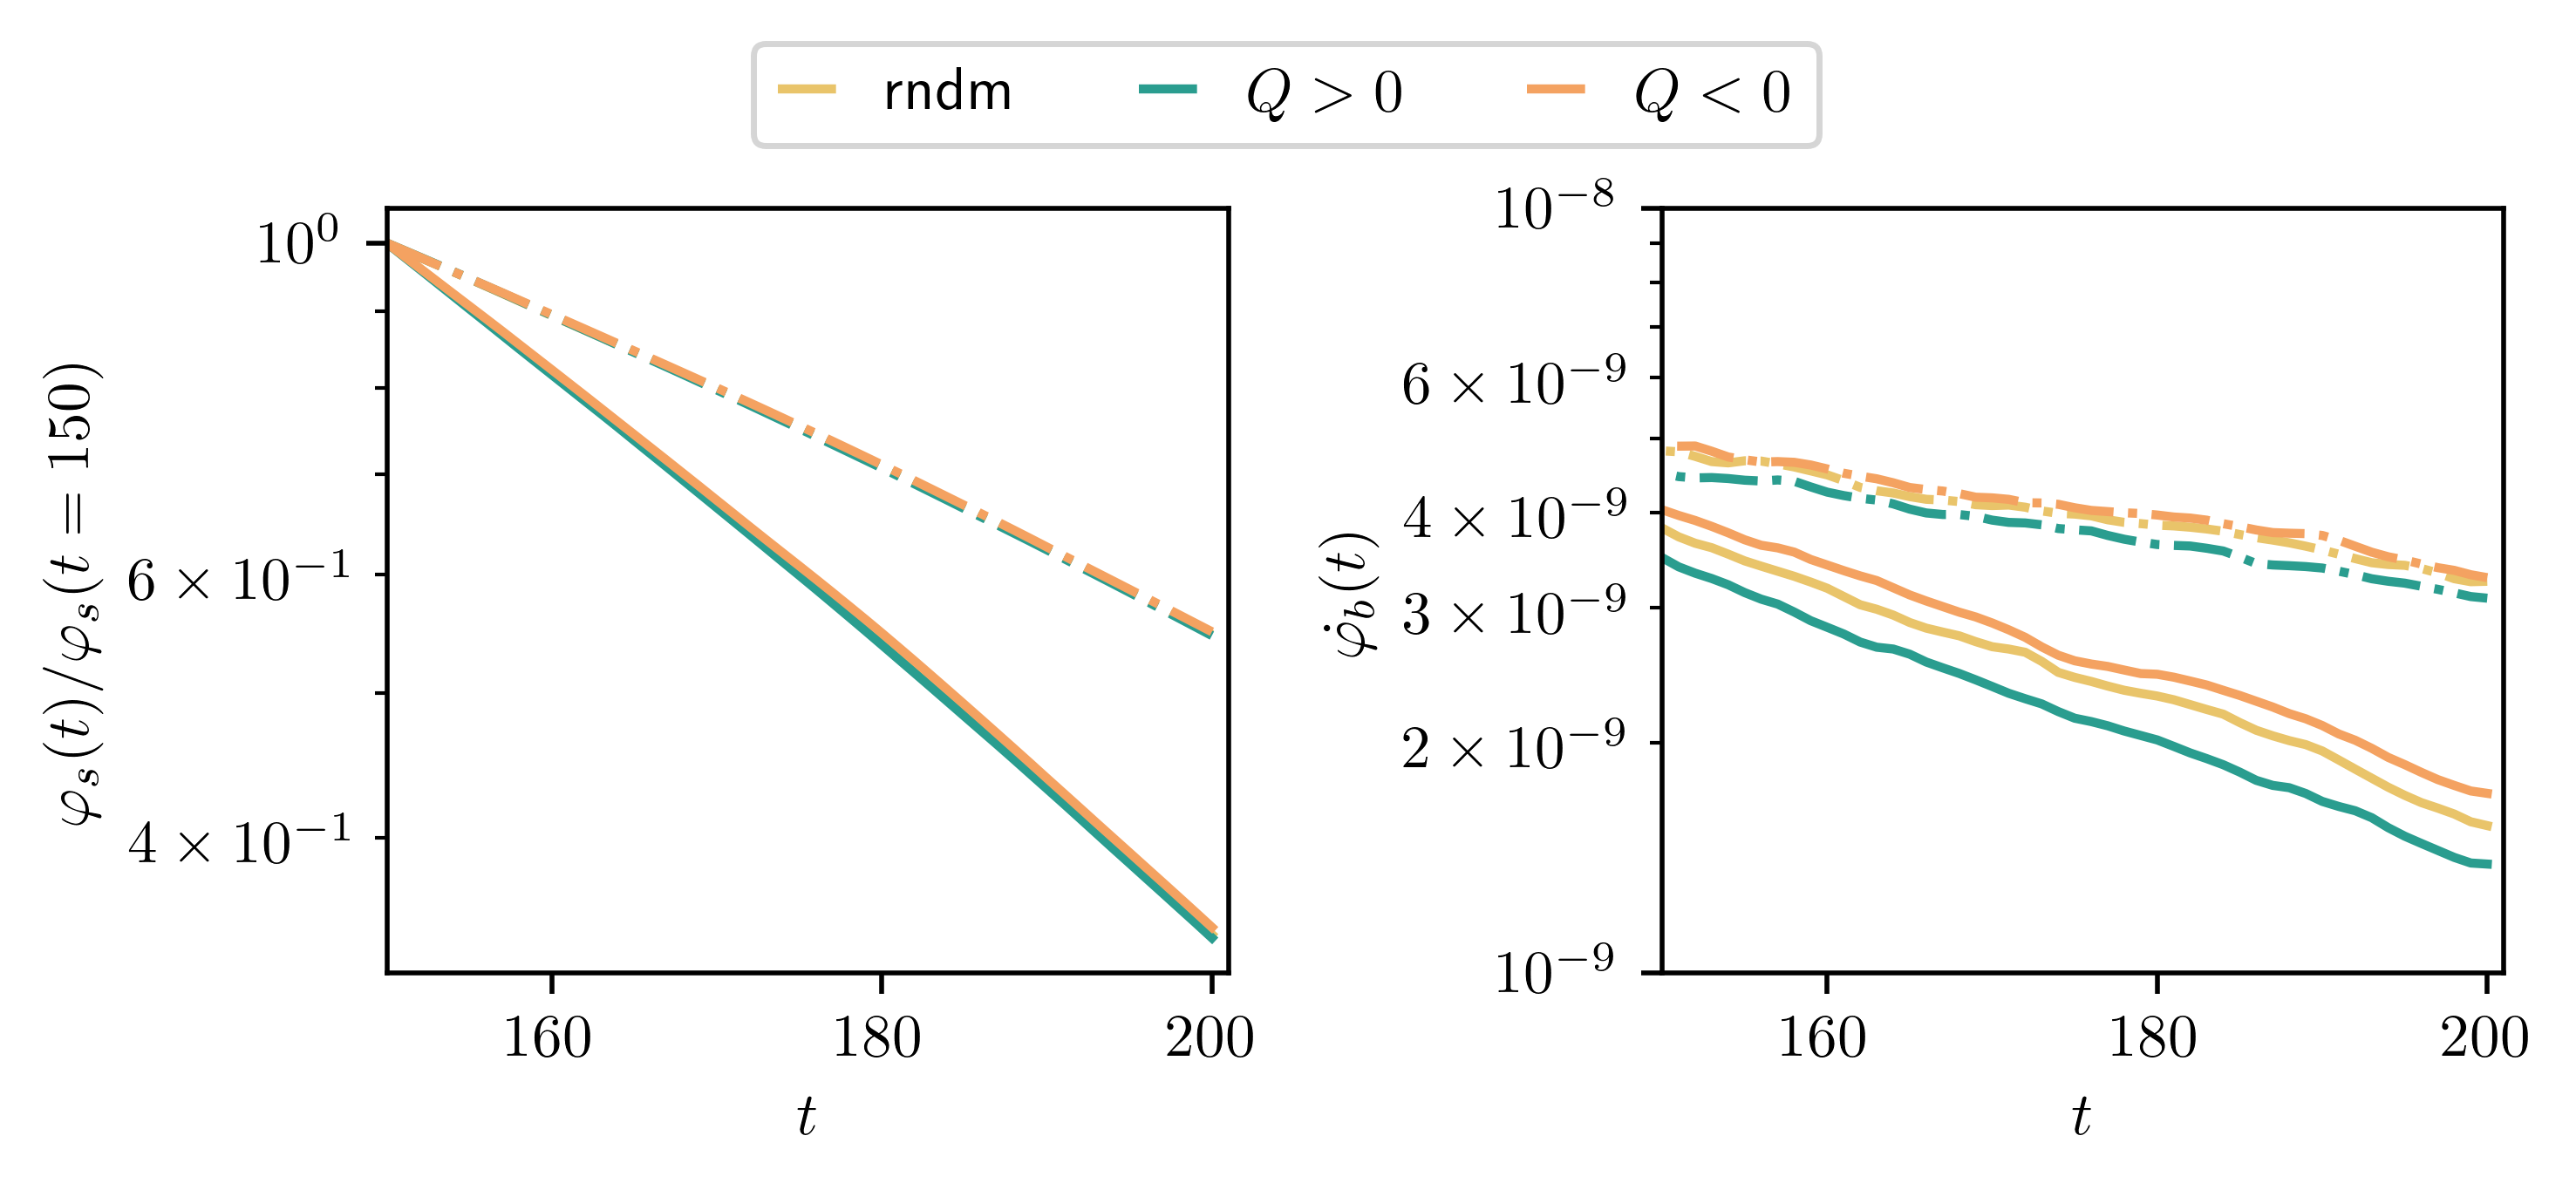
\includegraphics[width=\linewidth]{./figures/polydisperse/largetimes-2d.png}
	\end{center}
\caption[Late-time exponential decay of the droplet volume fractions]{(left) Volume fraction of small droplets at late times. It follows exponential decay. (right) Rate of change of volume fraction of large droplets calculated from local slope. As expected, it also follows exponential decay.}
\label{lucky-largetimes-2d}
\end{figure}


\section{Numerical Methods}
We will evolve the number density field in Eq. \eqref{mass-cont} pseudo-spectrally with phase-shifted $2\sqrt{2}/3$ dealiasing \cite{patterson1971} and periodic boundary condition. The Dirac-delta function is approximated with the cosine kernel at the locations of the big particles \cite{peskin2002} 
\begin{align}
\label{delta}
\begin{split}
    \delta(x-X) =\begin{dcases}
        \frac{1}{4h}\bigg\{1+\cos\left[\frac{\pi (x - X)}{2\Delta x}\right]\bigg\}, \ \ \ \ |x-X| \leq 2\Delta x,\\
        \   0 \ \ \ \ \ \text{otherwise},
        \end{dcases}
\end{split}
\end{align}
where $\Delta x = 2\pi/N_g$ is the resolution of the grid, and $\delta(\vec{x} - \vec{x}_0) = \delta(x - x_0)\delta(y - y_0)\delta(z - z_0)$. The background flow $\vec{u}$ is evolved pseudo-spectrally with phase-shifted $2\sqrt{2}/3$ dealiasing in periodic boundary condition according to the Navier-Stokes equation
\begin{align}
% \label{}
\begin{split}
    \frac{D \vec{u}}{Dt} = -\vec{\nabla}\mathcal{P} + \nu \Delta \vec{u} + \vec{F}_{\vec{u}}.
\end{split}
\end{align}
in $3$D. For $2$D, we adopt the evolution of chapter \ref{fn-cstcs} with vorticity obeying Eq. \eqref{int-2DNS}. 

The particles are evolved Lagrangially, and the background velocity $\vec{u}$, small particle number density $n$, and small particle velocity $\vec{v}_s$ are interpolated at the location of the particle using a cosine kernel method \cite{pandey2019}.
\begin{align}
% \label{}
\begin{split}
    \phi(\vec{x}_b,t) = \sum\limits_{\vec{x}\in \vec{x}_G}^{} \phi(\vec{x},t) \delta(\vec{x} - \vec{x}_b) (\Delta x)^3,
\end{split}
\end{align}
where $\phi$ is any field, scalar or vector, to be interpolated. 

The spectral evolution of number density does not ensure its positivity due to truncation. Therefore, at every step, we pass the number density through a filter which clips the negative values of number density to zero, and rescales the mean to ensure no mass is gained due to clipping. This does introduce some error, but this is the least erroneous thing to do in a spectral truncation. We have experimented with other forms of clipping and rescaling, and the details are given in Appendix \ref{clip-alt}.




\vspace*{1em}
\hrule
\vspace*{1em}



% \begin{table}
%     \centering
%     \renewcommand{\arraystretch}{2} % spacing between rows
%     \begin{tabular}{cccc}
%     \hline
%     \textbf{St} & \textbf{Init} & $\lambda_s$ \textbf{ left} & $\lambda_s$ \textbf{ right} \\ \hline
%     0.01 & rndm   & -0.02128 & -0.01720 \\
%     0.02 & rndm   & -0.01203 & -0.00760 \\
%     0.01 & $Q>0$  & -0.02134 & -0.01809 \\
%     0.02 & $Q>0$  & -0.01208 & -0.00770 \\
%     0.01 & $Q<0$  & -0.02101 & -0.01675 \\
%     0.02 & $Q<0$  & -0.01196 & -0.00744 \\ \hline
%     \end{tabular}
%     \caption[Fitted slopes for the late-time volume fractions]{Fitted slopes $\lambda_s$ for the left and right part of Fig. \ref{lucky-largetimes-2d}. They do not match.}
% \end{table}



% Now, although the growth rate for smaller initial $St_b$ are higher, do they produce droplets that cross a certain size threshold faster? The answer is YES! Suprisingly, the drops with larger initial $St_b$ has slower growth due to smaller number of particles, each of those particles gets to eat up a lot of small droplets and grow faster. Figure \ref{lucky-thresh} demonstrates this phenomenon.

% \begin{figure}
% 	\begin{center}
% 		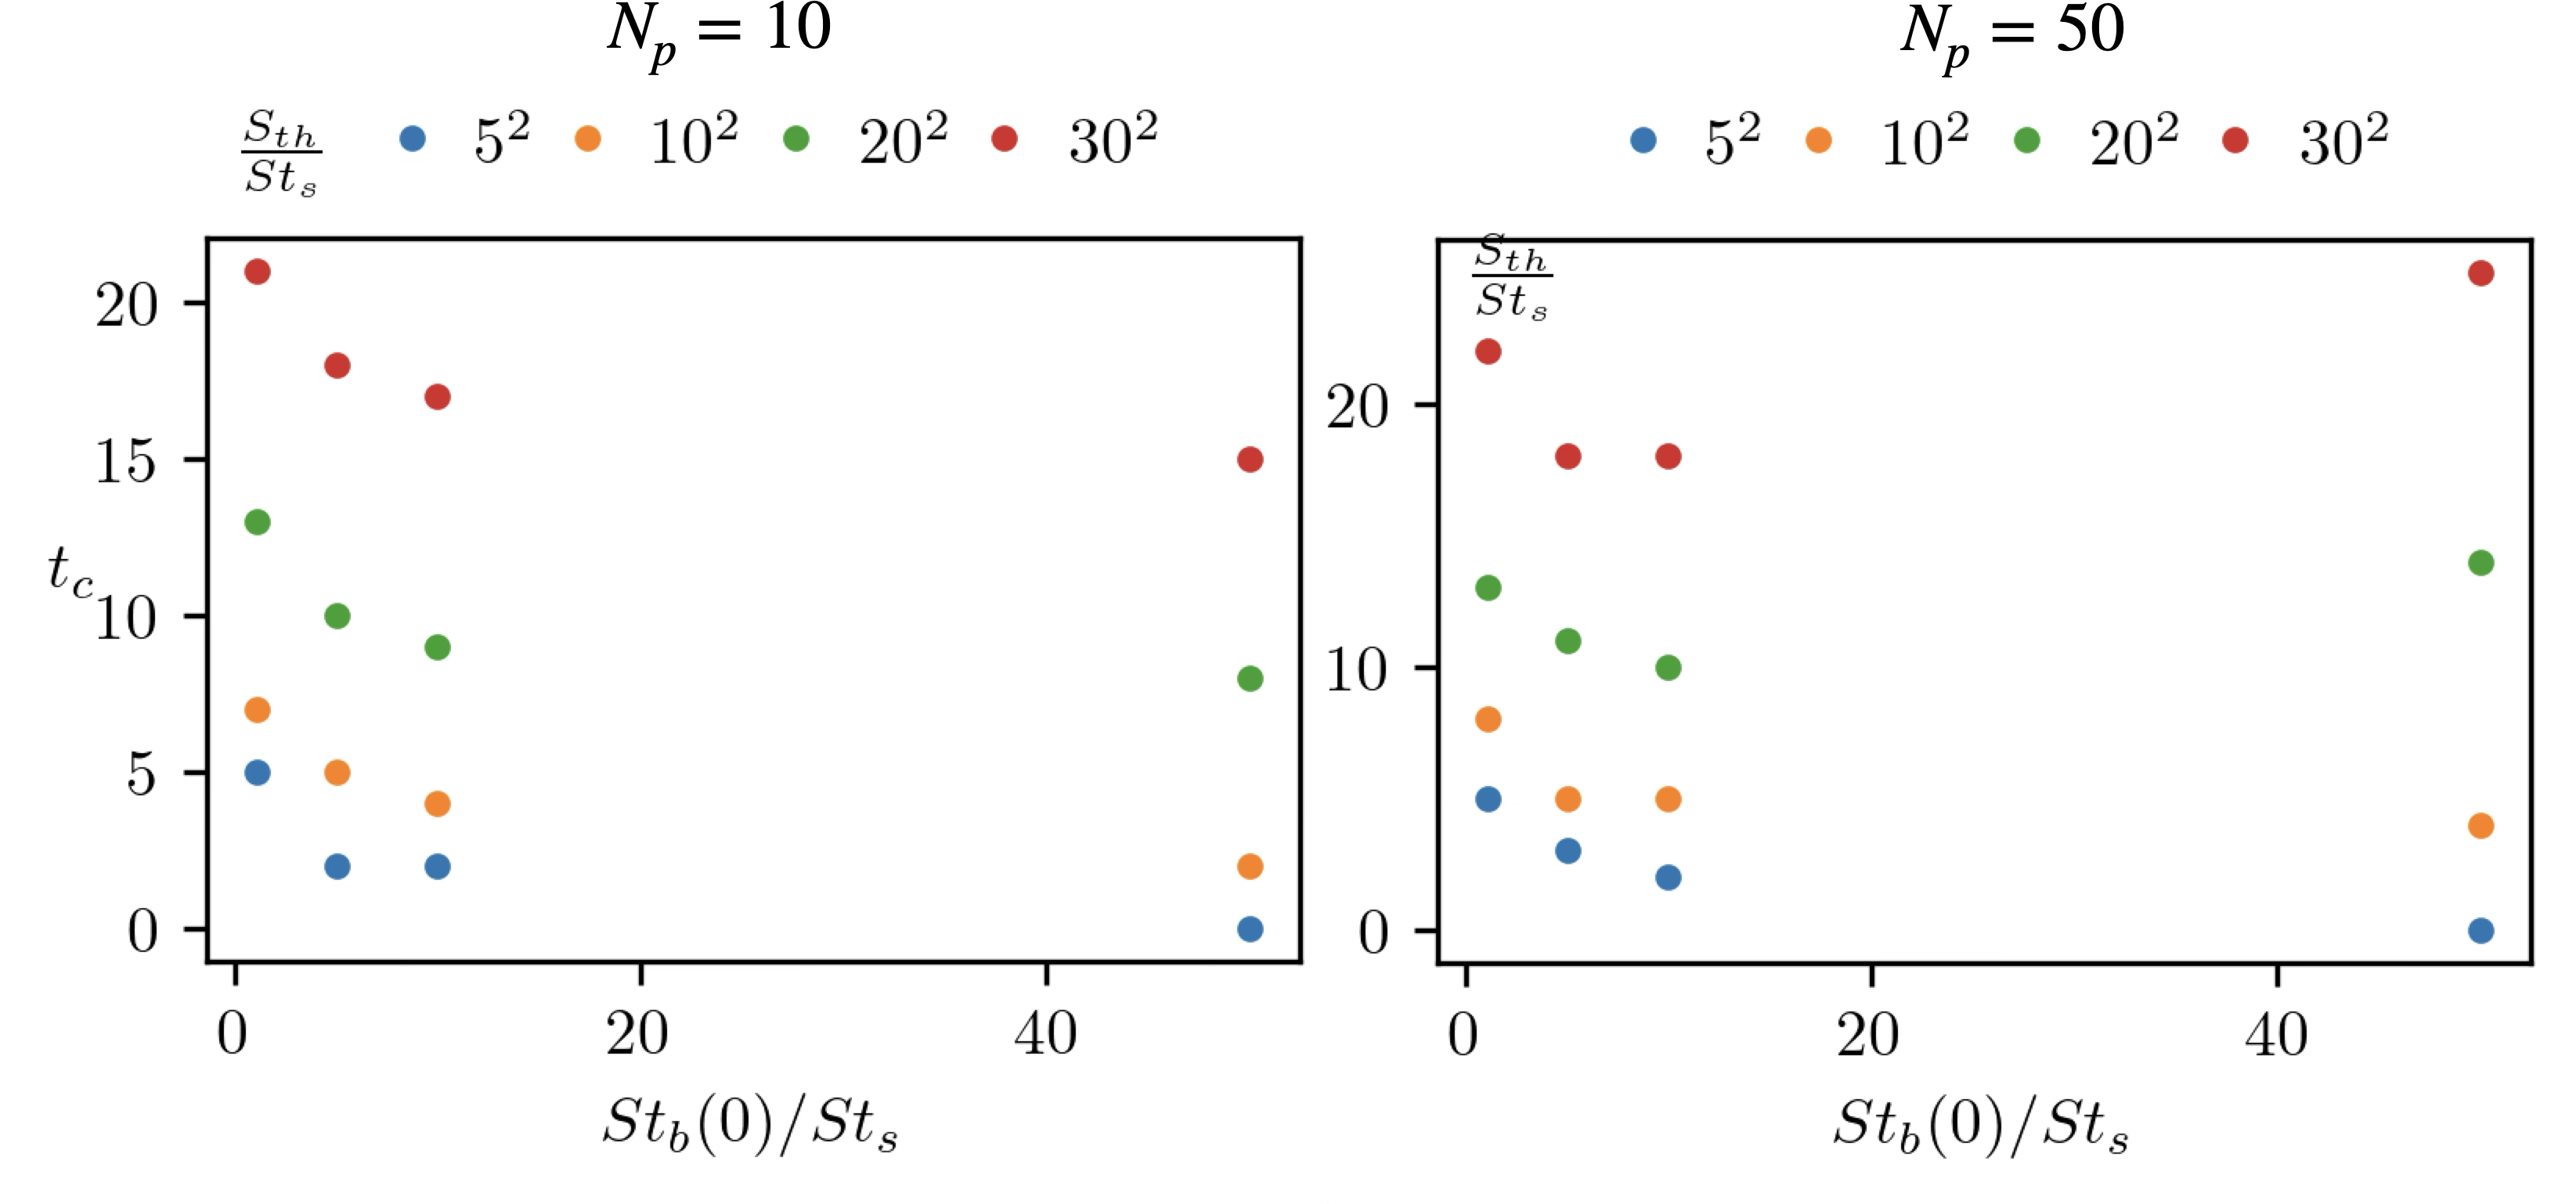
\includegraphics[width=\linewidth]{./figures/polydisperse/threshold-growth.png}
% 	\end{center}
% \caption[Time for big droplets to grow past a threshold]{Time taken for 10 particles (left) and 50 particles (right) to grow beyond a certain threshold for different initial $St_b$s}

% \label{lucky-thresh}
% \end{figure}

% \begin{figure}
%     \centering
%     % \import{/Users/rajarshi/Library/CloudStorage/GoogleDrive-rajarshi.chattopadhyay@icts.res.in/My Drive/Collab/plots/Re_125000.0,dt_0.005,N_1024/sts_0.005_stb_0.30/time_100.0}{sm-10000big.pgf}
%     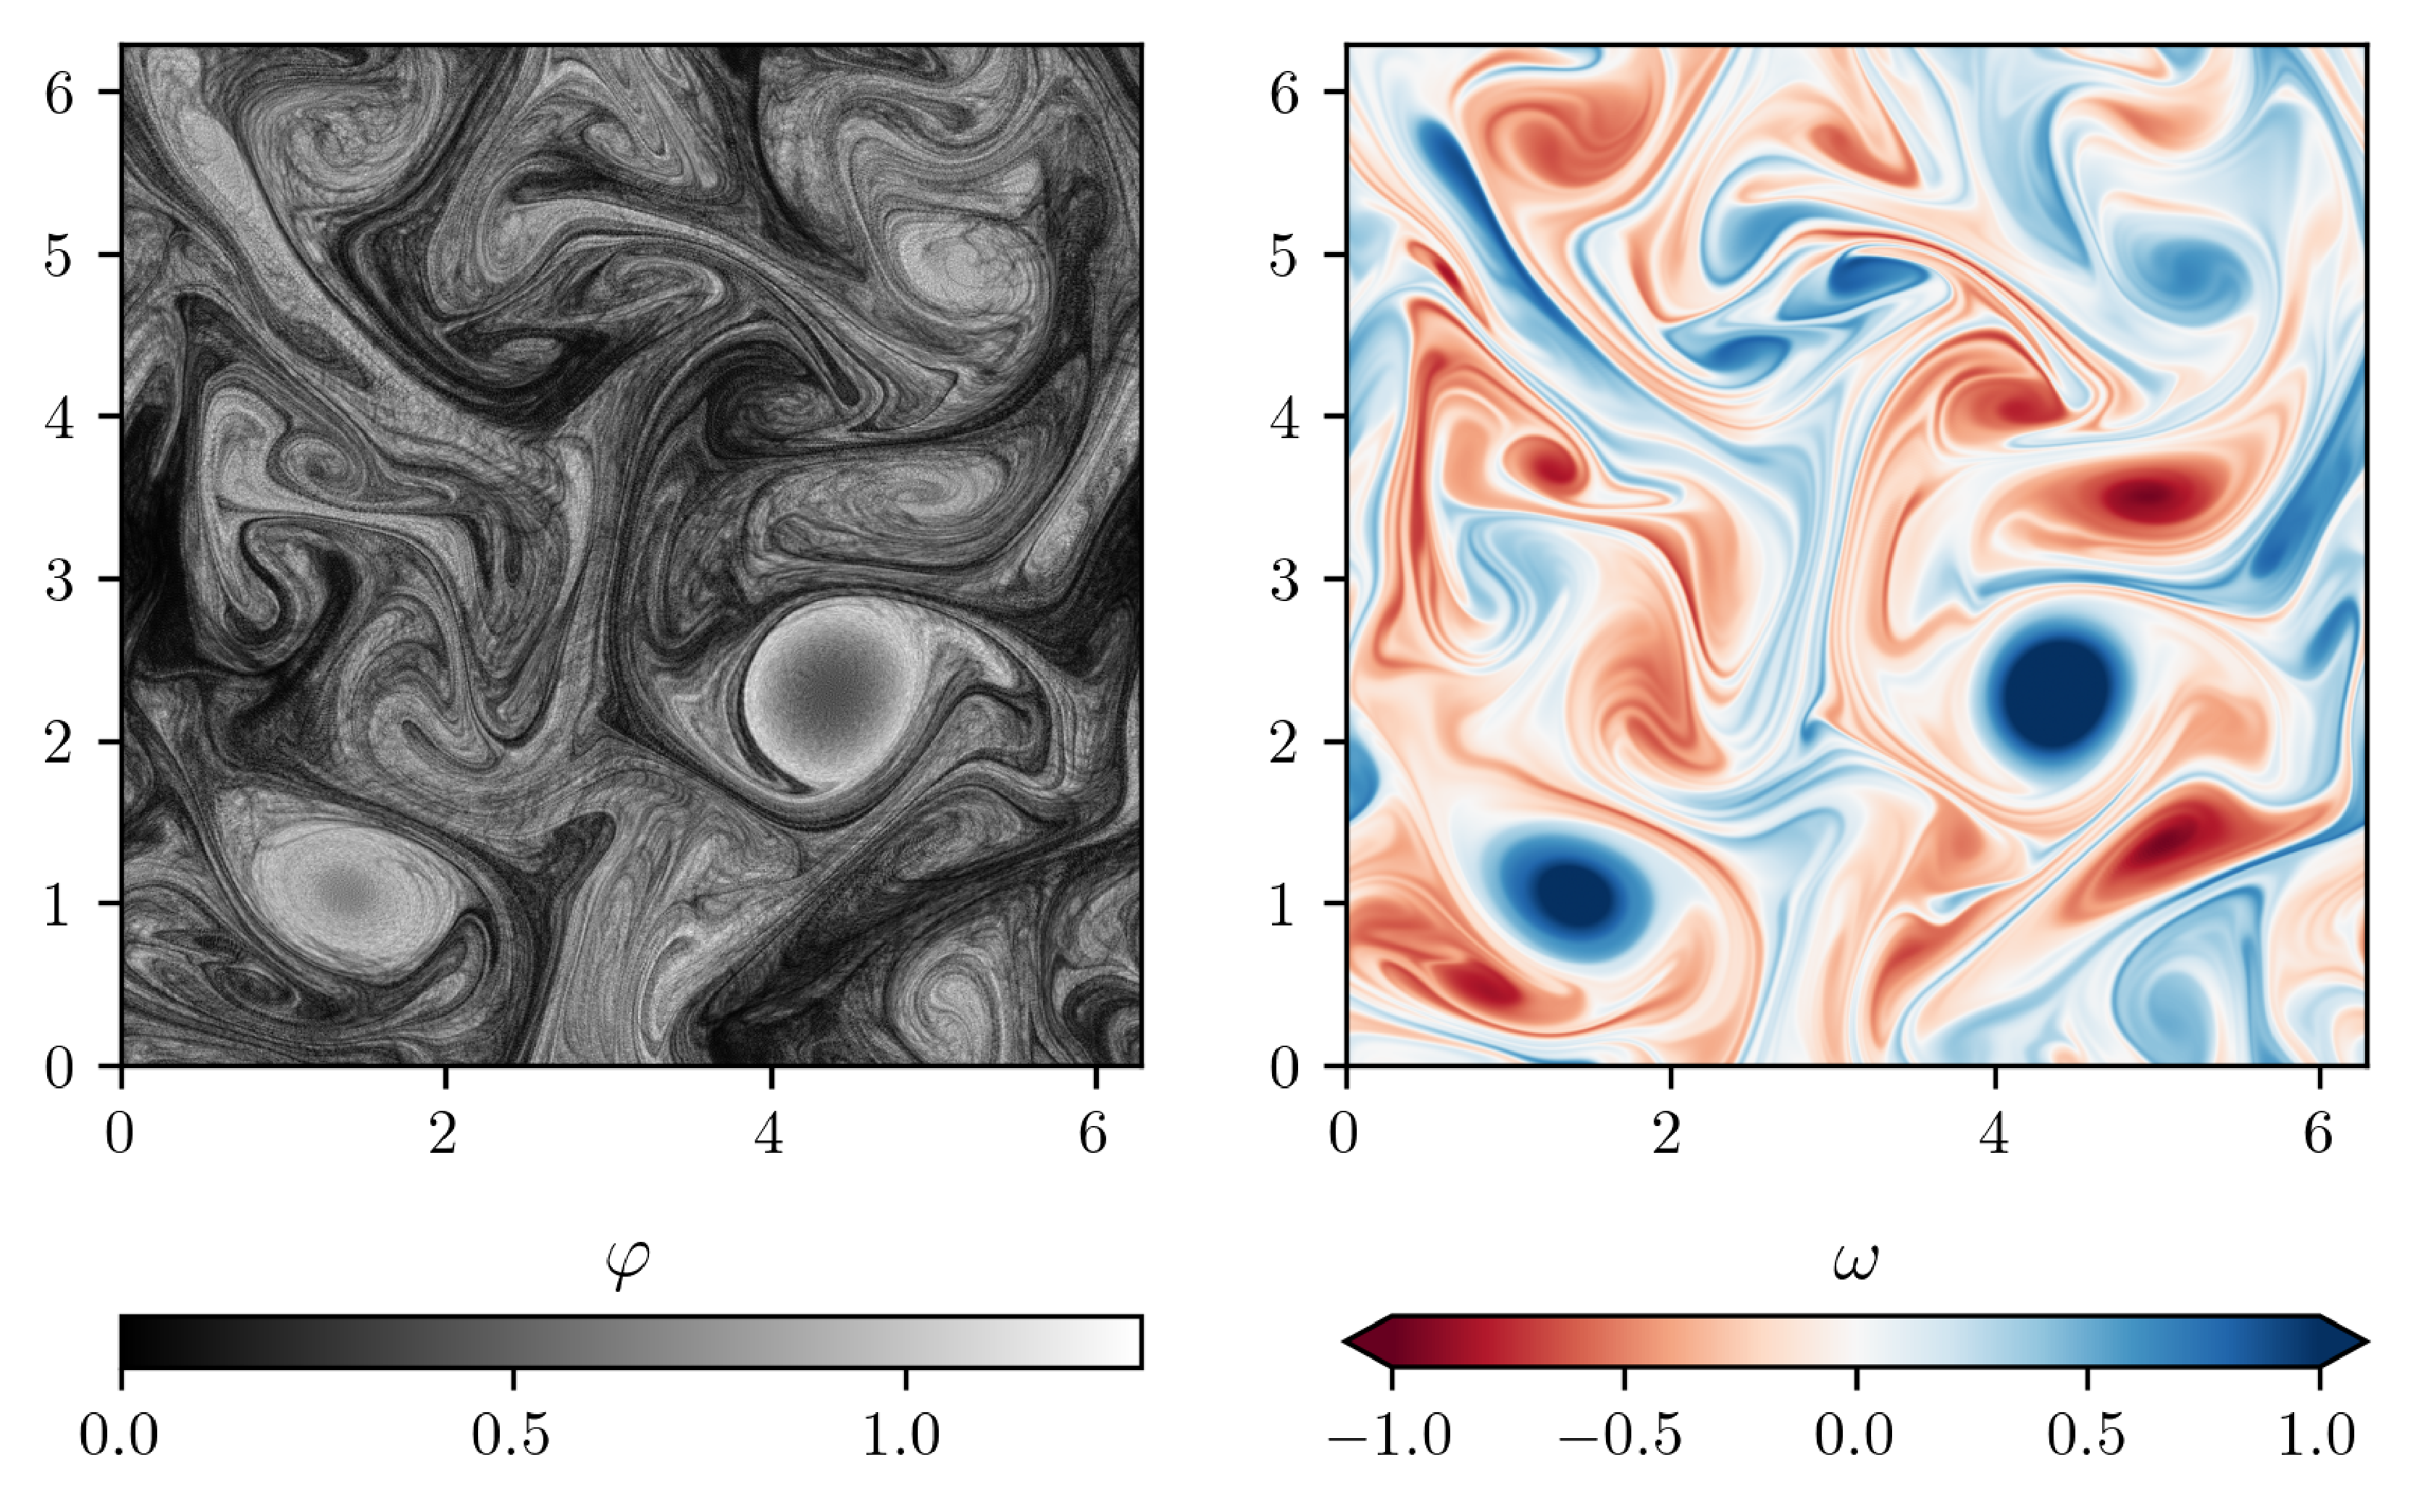
\includegraphics[width=\linewidth]{./figures/polydisperse/sm_0.02_0.002.pdf}

%     \caption[Vorticity and small-droplet volume fraction with one big droplet]{Instantaneous snapshot showing the vorticity of the $2$D flow (right) along with the small particles's volume fraction (right) normalized by the mean volume fraction. The small white streaks are the places from where the big particle have run through.}
%     \label{lucky-zeta-sm-1big}
% \end{figure}

% \begin{figure}
%     \centering
%     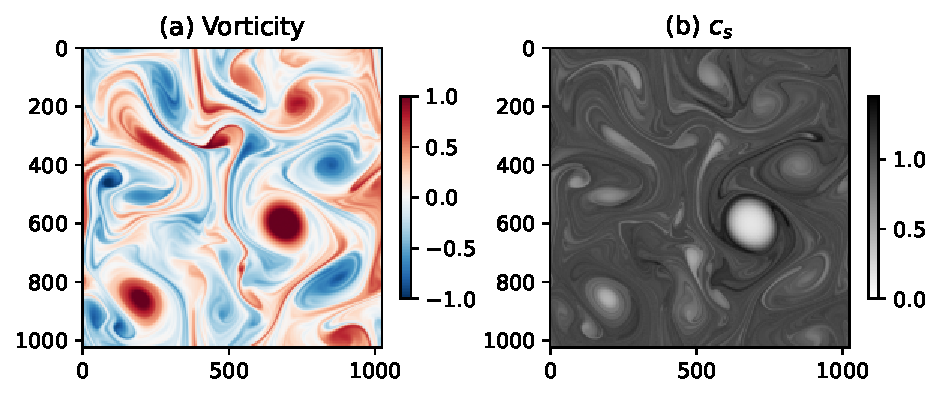
\includegraphics[width=\linewidth]{./figures/polydisperse/sm-nobig.pdf}
%     \caption[The same snapshot without any big droplet]{Same as in \ref{lucky-zeta-sm-1big} without any big particle. No such small streaks exist in the small particle's number density. }
% \end{figure}

For a $1m^3$ cumulus cloud with $10^9$ $10\mu m $ droplets, the net volume fraction occupied is $\sim 4\times 10^{-6}$. Thus, the mean volume fraction, $\langle c_s \rangle$, for a cloud ranges between $10^{-5}$ to $10^{-6}$. That is a reference number we will put in our studies.

For extrapolating on the grid, we are using the mechanism of \citep{pandey2019}.


% \section{Lagrangian studies}
% If one simulates individual particles, they investigate the quantity $P(m,t)$, probability density of a particle of mass $m$ at time $t$. As mass is \emph{assumed to be } conserved at each collision, it is a good index in tracking particles. The evolution equation of $P(m,t)$
% \begin{align}
% % \label{}
% \begin{split}
%     \dot{P}(m,t) = \jin{m,t}-\jout{m,t}\ ,
% \end{split}
% \end{align}
% where $\jin{m,t}$, and $\jout{m,t}$ are the influx and outflux of particle probability of size $m$. It makes sense that $\jin{m.t}$ is made up of collision between all the particles that results in a particle of size $m$, and similarly $\jout{m,t}$ consists of all the collisions between particles of size $m$ and others. Thus,
% \begin{align}
% % \label{}
% \begin{split}
%     \jin{m,t} &= \int\limits_{m' = 0}^{m} \lambda(m',m - m', t)P(m',t)P(m-m',t) \\
%     \jout{m,t} &= P(m,t)\int\limits_{m' = 0}^{\infty} \lambda(m,m', t)P(m',t) \ ,
% \end{split}
% \end{align}
% where $\lambda(n,m,t)$ is the rate of collision between particles of mass $m$ and mass $n$ at time $t$. This inherently leads to nonlinearity of the probability density evolution. \texttt{Note that this disregards collisions of $3$ or more particles.} The rate of collision, also measures the survival probability $S(m,t)$ of a single particle.
% \begin{align}
% % \label{}
% \begin{split}
%     \dot{S}(m,t) = - S(m,t)\int\limits_{m' = 0}^{\infty} \lambda(m,m', t)P(m',t) \ .
% \end{split}
% \end{align}
% Thus, if we define $\varLambda(m,t)= \int\limits_{m' = 0}^{\infty} \lambda(m,m', t)P(m',t) $ as the rate of collision of a particle of size $m$ with particles equal or larger than its size, then,
% \begin{align}
% % \label{}
% \begin{split}
%     S(m,t) = S(m,0)~\exp\left(-\int\limits_{t' = 0}^{t}\varLambda(m,t')\right) \ .
% \end{split}
% \end{align}



% \citet{batge2026} simplified the fluxes by considering \emph{theoretically} that all the collisions are between the smallest particles with $m = 1$. Furthermore, the concentration of these small droplets also do not change with time, i.e., $P(1,t) = P(0,t)$. Although these assumptions raise doubts, they get \textbf{decent} agreement with numerical results.


% Now, knowing $P(m,t)$ allows one to calculate how much time would it take to have a certain probability of  formation of droplet of size $m = M$. But to evolve the equation, one needs to know $\lambda(m,m',t)$. \citet{batge2026} and \citet{bec2016} found those differently, and those are valid in different regimes.
% However, a lower level idea is $P(m,x,t)$, distribution of droplets at each location. \emph{This is not captured by any Lagrangian simulations so far.} \texttt{Maybe Frederik Gareis will do it?}

% \begin{description}
%     \item[Growth rate in continuum limit] In our hybrid simulations, growth rate of each particle is exactly known form Eq. \eqref{lucky-2Deqns} and  \eqref{lucky-3Deqns}. Can we use it capture the growth rate of the Lagrangian simulations?
%     \item[Evolution of $P(m,t)$] In the continuum limit, the size of each big particles change at each instant, then how does one consider the \texttt{in} and \texttt{out} fluxes?
%     \item[Maybe evolving $P(m,t)$ is not the goal] In the continuum limit, $P(m,t)$ is found by binning the particles at each instant. The number of big particles never change, thereby preserving the total number of big particles. How does this additional constraint help?
%     \item \textbf{Is there a quantity that can be calculated both from the Eulerian and the Lagrangian perspective apart from the evolved $P(m,t)$?}
% \end{description}

\section{2D Results}

We run our numerical simulation for the following parameters.
\begin{table}
    \centering
    \begin{tabular}{|ccccccc|}
    \hline
        Runs & $V_s(0)$  & $V_b(0)$ & $St_s$ & $St_b(0)$& $\alpha_g$ & \\
        \hline
        1& $10^{-6}$ & $10^{-9}$ &0.005  &0.3 & & \\
        2& $10^{-6}$  & $10^{-9}$ &0.01  & 0.3 & & \\
         3& $10^{-6}$ & $10^{-9}$ &0.02  &0.3 & & \\
         \hline
    \end{tabular}
    \caption[Parameters of the different runs]{Parameters of the different runs. The growth rate of the big particles is fitted with $t^{\alpha_g}$}
    \label{lucky-tab:my_label}
\end{table}
% \begin{figure}
% 	\begin{center}
% 		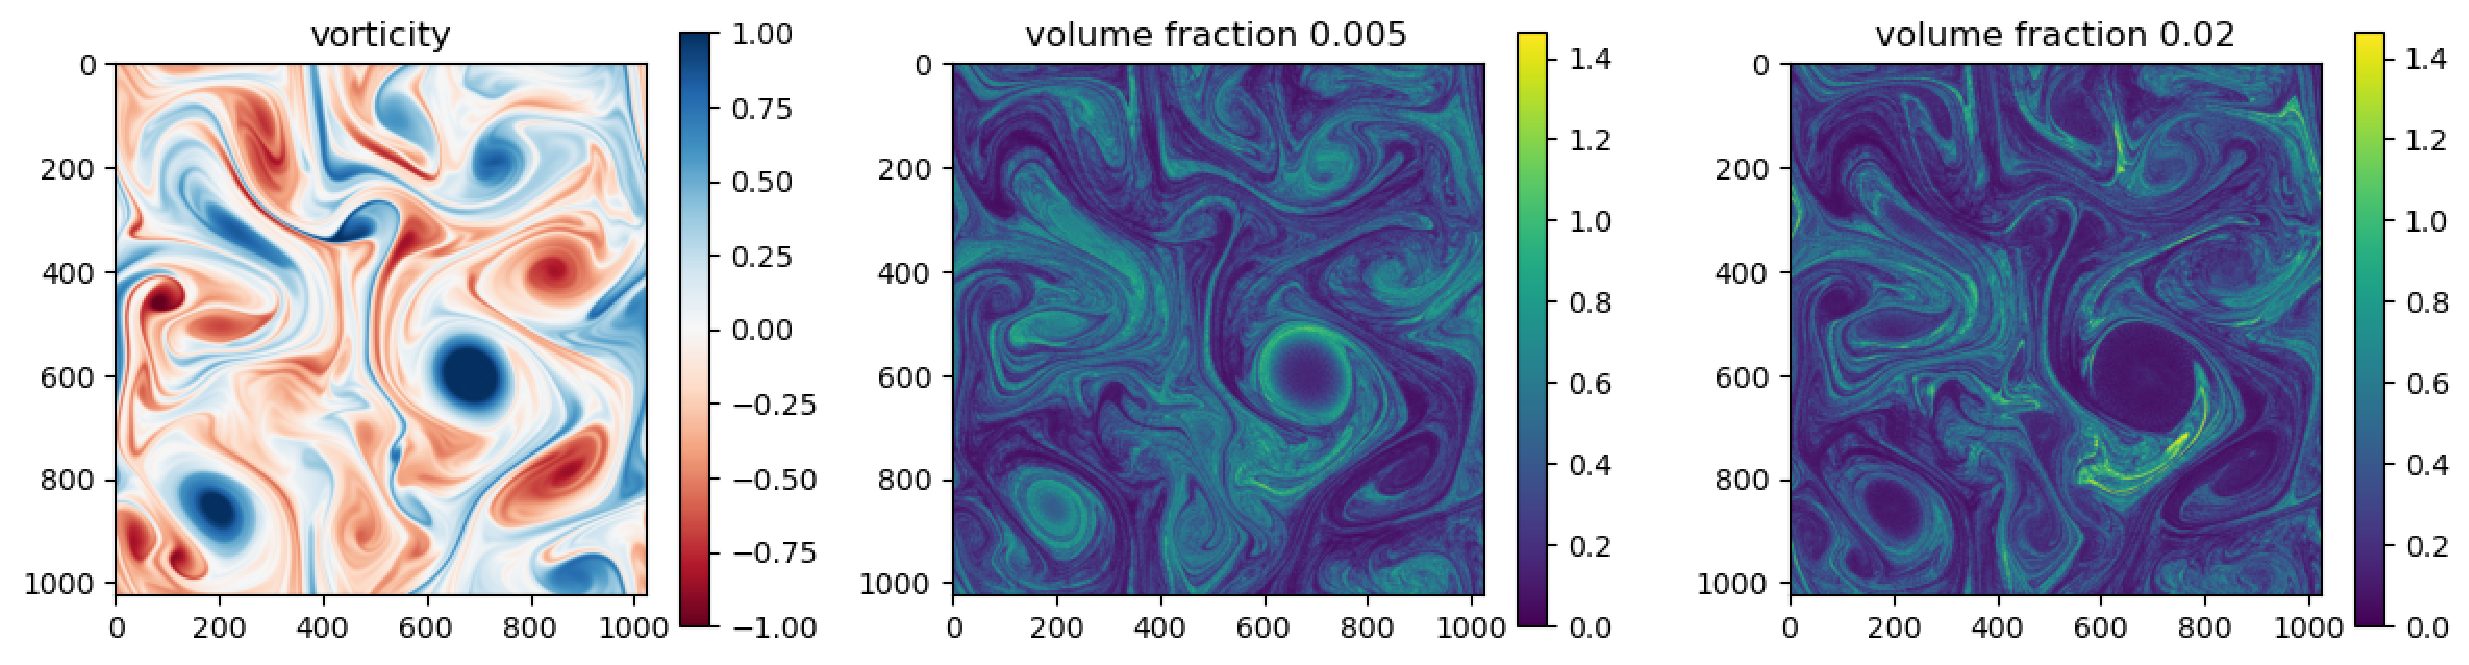
\includegraphics[width=\linewidth]{./figures/polydisperse/pstruc.pdf}
% 	\end{center}
% \caption[Depletion of small droplets at two Stokes numbers]{Volume fraction of the small particles evolved in presence of 10000 big particles for runs 1 (middle) and 3 (right). We see larger Stokes small particles get more depleted or eaten up by the big particles.}
% \label{lucky-pstruc}
% \end{figure}
For runs 1 and 3, we check the growth rate of particles starting from regions of positive and negative $Q$. Regions of positive $Q$ represents vortical regions while negative $Q$ represents strain regions. We find particles starting out in vortical regions grow larger at later time, Fig. \ref{lucky-grth-diffQ}.
% \begin{figure}
% 	\begin{center}
% 		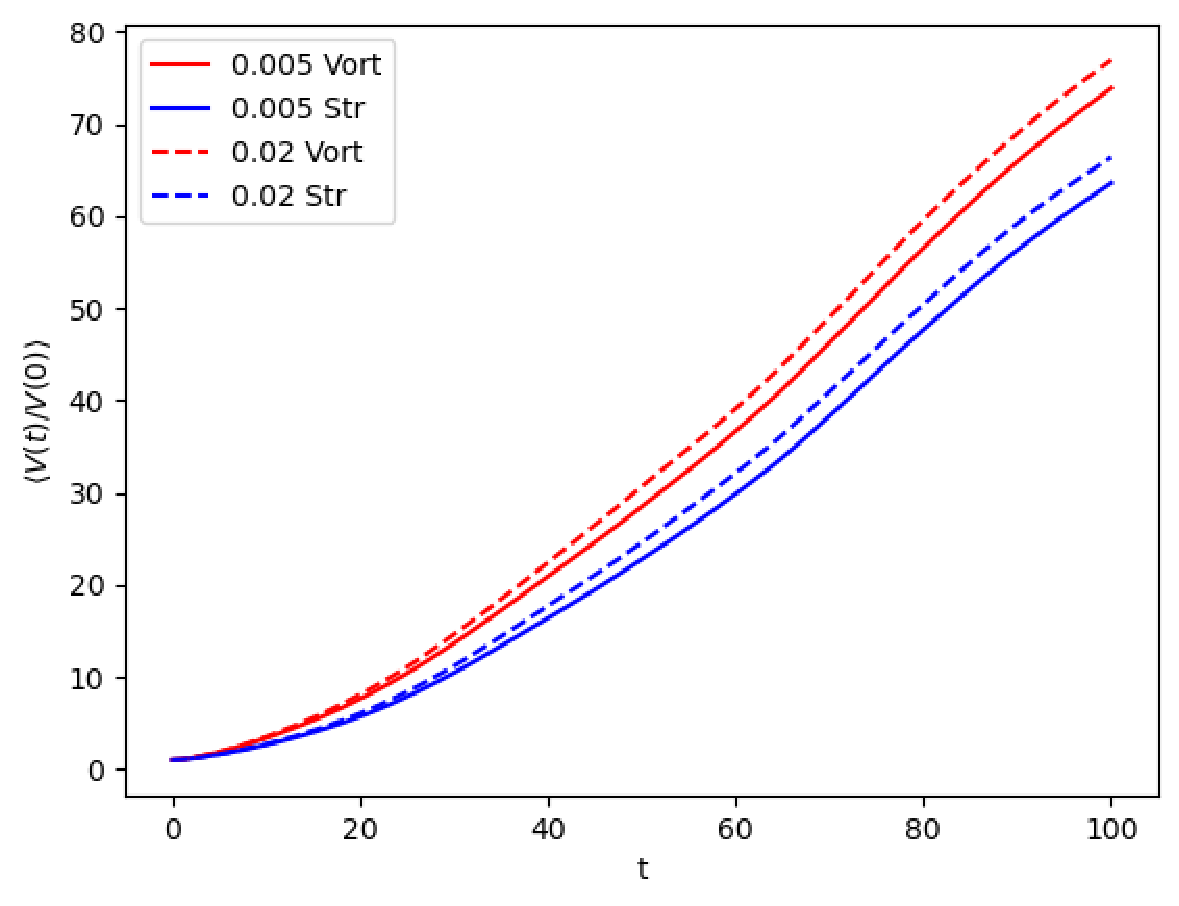
\includegraphics[width=0.6\linewidth]{./figures/polydisperse/diff-Q-grwth-rate.pdf}
% 	\end{center}
% \caption[Growth rate of big droplets starting in vortical and strain regions]{Growth rate of big particles starting in positive and negative $Q$ regions for runs $1$ and $3$ with 10000 big particles. Particles starting out in the vortical region experience a larger growth rate. Furthermore, the growth rate increases significantly upon increasing the $St$ of small particles.}
% \label{lucky-grth-diffQ}
% \end{figure}

Next, we try to see whether particles start gaining more liquid content if they encounter a strong vortex. For that we consider particles that have encountered vortices stronger than $2\zeta_{\rm rms}$, where $\zeta_{\rm rms}$ is the root-mean-square vorticity of the background field.

% \begin{figure}
% 	\begin{center}
% 		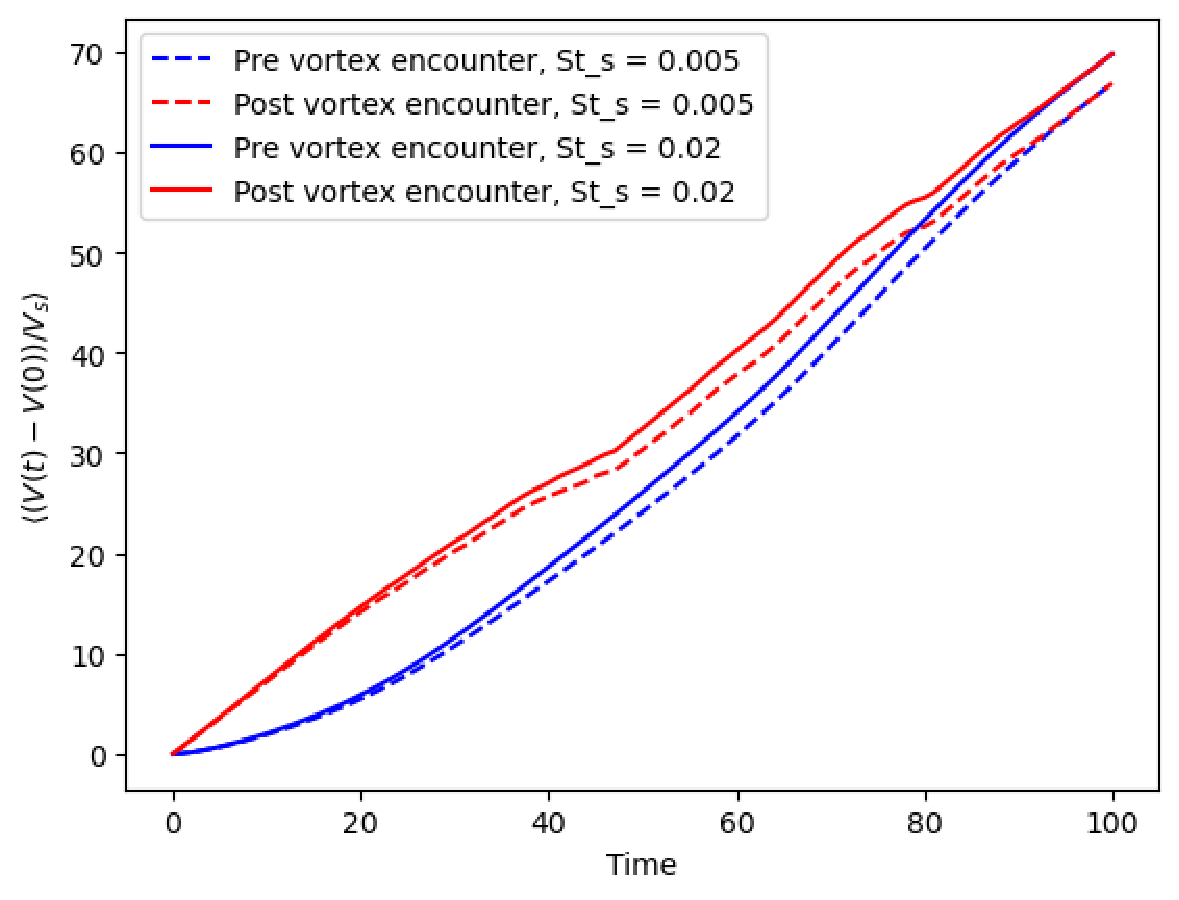
\includegraphics[width=\linewidth]{./figures/polydisperse/pre-post-vort.pdf}
% 	\end{center}
% \caption[Volume gained by big droplets passing through high vorticity]{Volume gained by the big particles that went through a region of big vorticity.}
% \label{}
% \end{figure}
At early times, right after entering the vortex, we see that the big particles grow much larger. This may be because of two reasons. First, only the particles that are big enough to significantly avoid streamlines enter these big vortical regions. These particles already being bigger than the rest, naturally accumulate more small particles owing to their larger collision cross-section. However, this effect should also be there at late times, but we see that the growth rate slow down. The second reason is also an interesting one. Larger particles get centrifuged out more out of the large vortical regions. On their way out, these particles are prone to capture many small particles.
Next, we want to study the growth rate within the vortical region. To do so, we track when a big particle enters and leaves a big vortex $\zeta > 2\zeta_{\rm rms}$ and plot the volume grown as a function of the residence time. Apriori, we do not expect significant growth \emph{inside} the vortex, but rather after they come out of a big particle.

\section{Initial conditions of the `Lucky' Particles}
If we seed the lucky droplets uniformly in the domain, and evolve, the first and the last stage is given below.
% \begin{figure}
% 	\begin{center}
% 		\includegraphics[width=0.9\linewidth]{./figures/polydisperse/rndm_0.002_0.02.pdf}
% 	\end{center}
% \caption[Fate of small droplets for randomly placed lucky droplets]{Initial and final fate of the small particle concentration along with vorticity when `lucky' particles are initialized randomly over the domain. $St_b = 0.02$, $St_s = 0.002$. }
% % \label{}
% \end{figure}

Instead, if we initialize particles from the strongest vortex cores, we get the following,
% \begin{figure}
% 	\begin{center}
% 		\includegraphics[width=0.9\linewidth]{./figures/polydisperse/Qpos_0.002_0.02.pdf}
% 	\end{center}
% \caption[Fate of small droplets for lucky droplets started in high $Q$]{Initial and final fate of the small particle concentration along with vorticity when `lucky' particles are initialized in regions $Q> 3Q_{\rm rms}$. $St_b = 0.02$, $St_s = 0.002$. }
% \label{}
% \end{figure}
What happens to the growth rate of the `lucky' droplets? Do the ones starting out from the vortex core grow faster?
% \begin{figure}
% 	\begin{center}
% 		\includegraphics[width=\linewidth]{plots/grwth_rndm_Qpos_0.002_0.02.pdf}
% 	\end{center}
% \caption{Comparison of the evolution of the volume fraction of small and big particles as one changes the initial conditions. $St_b = 0.02$, $St_s = 0.002$.}
% % \label{}
% \end{figure}


If the volume fraction of the smaller droplets decay exponentially, then a relevant timescale is this decay timescale.

And finally, the size distribution captured by the distribution of the $St_b$ will be quite different.
% \begin{figure}
% 	\begin{center}
% 		\includegraphics[width=\linewidth]{plots/p(st_b)_0.002_0.02.pdf}
% 	\end{center}
% \caption{Final distribution of Stokes number for different initial condition.}
% % \label{}
% \end{figure}

\begin{figure}
	\begin{center}
		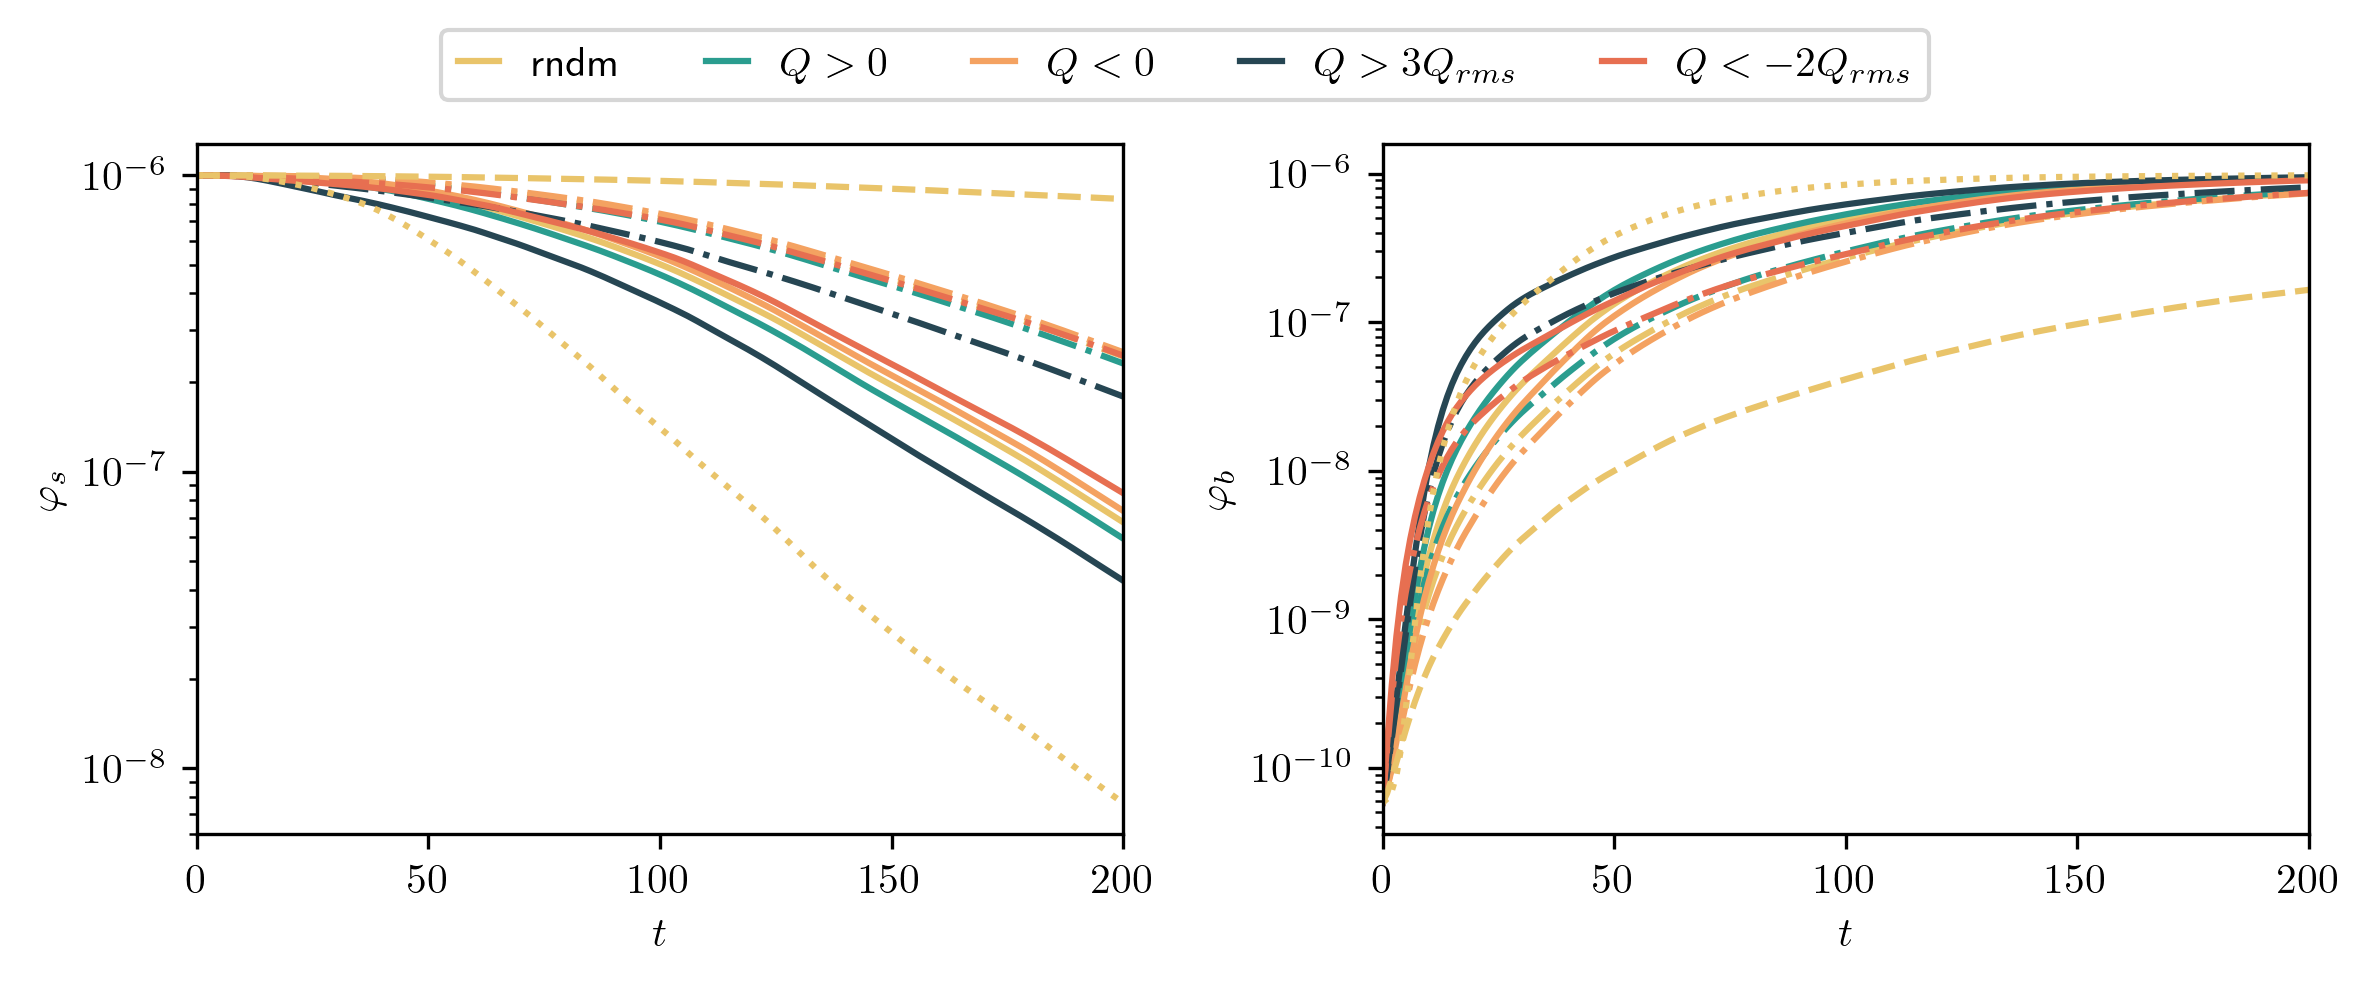
\includegraphics[width=\linewidth]{./figures/polydisperse/sts_0.002_stb_0.01,0.02_grwth.png}
	\end{center}
\caption[Growth of big droplets and decay of small droplets]{Growth rate of big particles (left) and decay rate of small particles (right), as one varies initial condition and Stokes numbers. Solid lines with $St_b(0) = 0.01$ and dashdotted lines with $0.02$. The dotted lines and the dashed lines are extreme Stokes numbered big particles with $St_b(0) = 0.0022$ and $St_b(0) = 0.1$, respectively. $St_s = 0.002$}
\label{lucky-grwth}
\end{figure}
\begin{figure}
	\begin{center}
		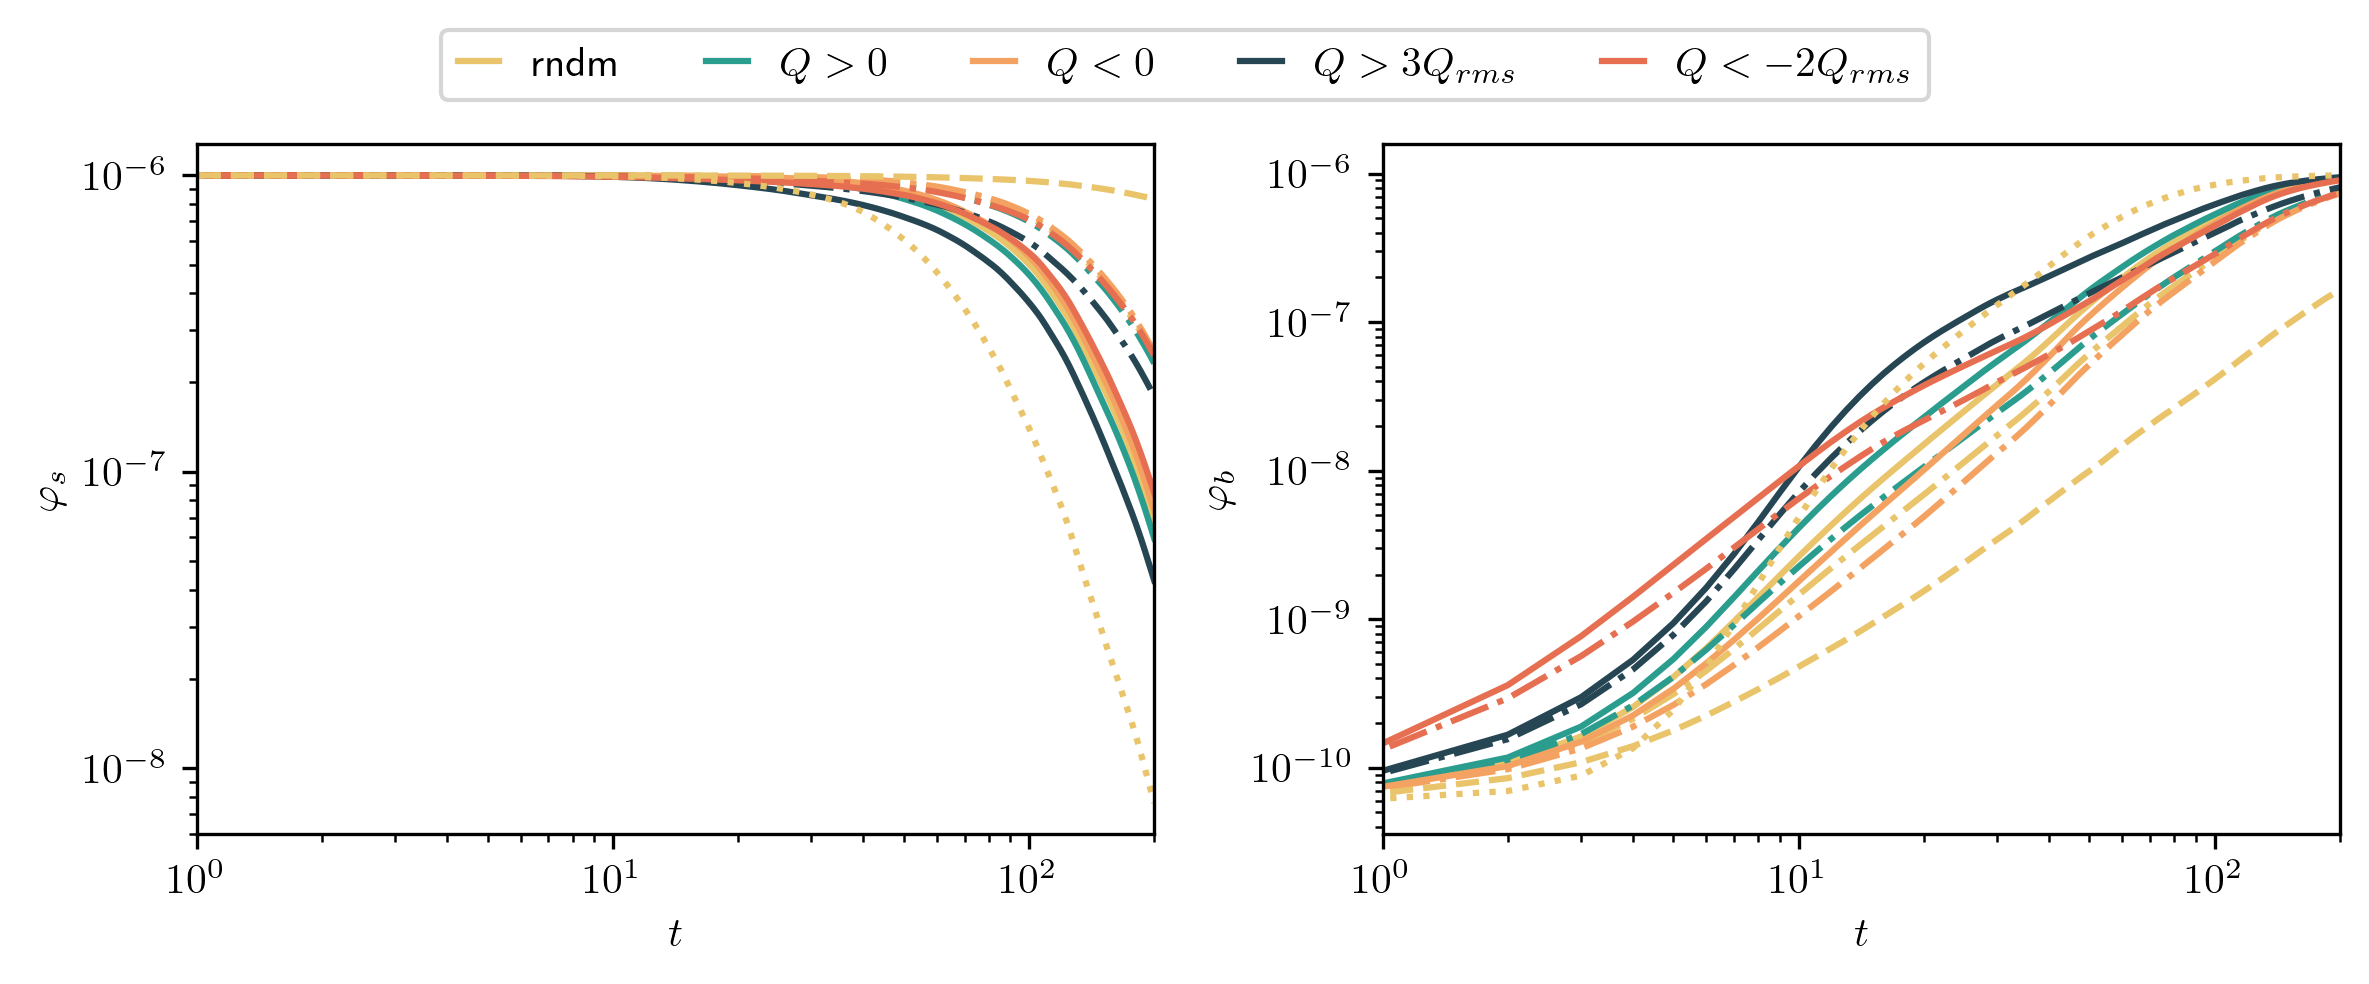
\includegraphics[width=\linewidth]{./figures/polydisperse/sts_0.002_stb_0.01,0.02_grwth_loglog.png}
	\end{center}
\caption[The same growth and decay rates on a log-log scale]{Same as \ref{lucky-grwth}, but in log-log scale.}
% \label{}
\end{figure}

\begin{figure}
	\begin{center}
		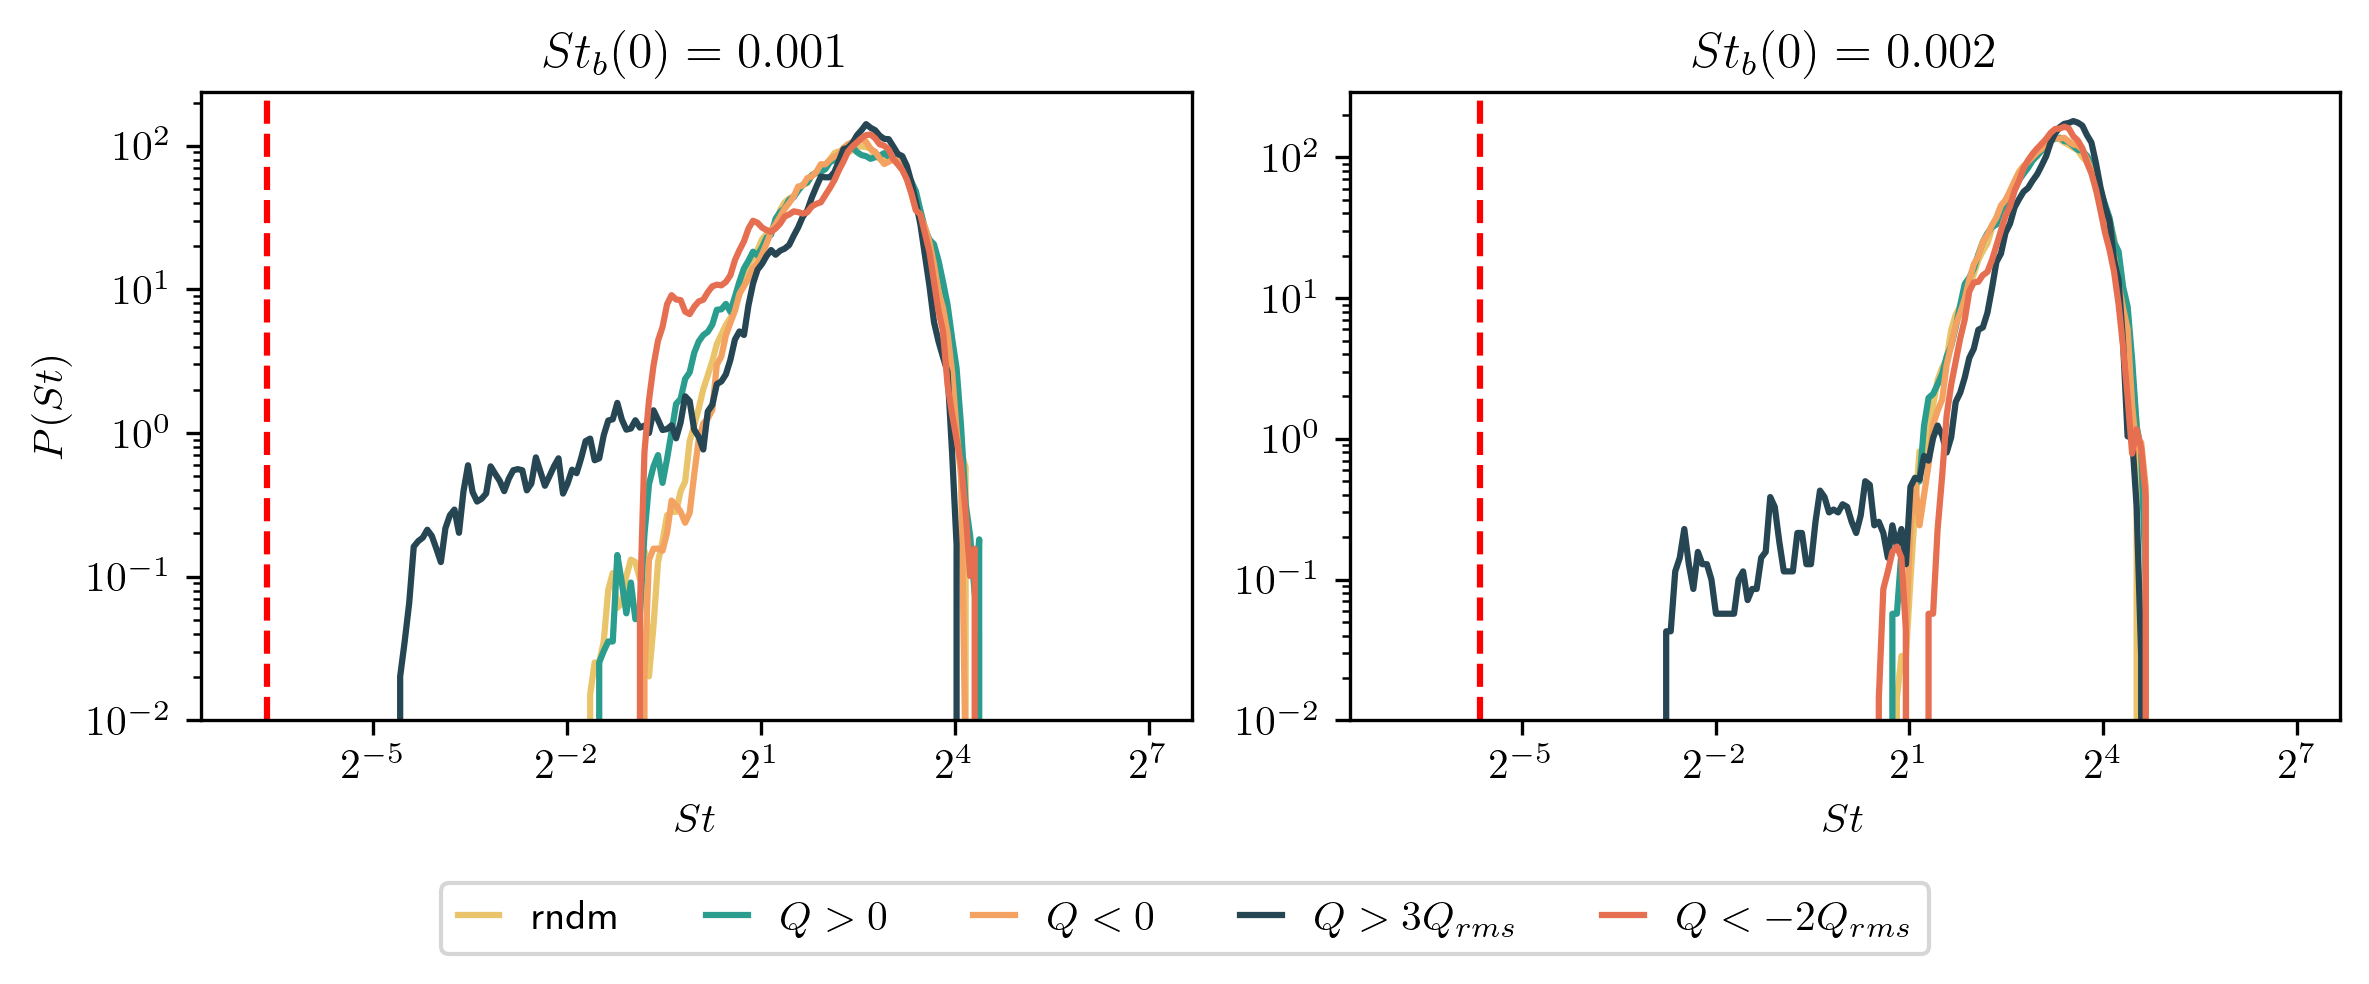
\includegraphics[width=\linewidth]{./figures/polydisperse/sts_0.002_stb_0.01-0.02_final_distribution.png}
	\end{center}
\caption[Final distribution of Stokes numbers for two initial values]{Final distribution of Stokes numbers with $St_b(0) = 0.01$(left), and $0.02$(right).$St_s = 0.002$}
\label{lucky-grwth-loglog}
\end{figure}

% \subsection{Possible limits of the growth rate}

% Here we try to describe and compare the possible limits of the growth rates. Remember, the mass absorbed by any lucky droplet particle is proportional to the size of the lucky droplet, the concentration of small droplets at the location of the lucky droplet, and the relative differences between the velocity of the lucky droplet and the local velocity of the small droplets. The complicated interplay of all these factors gave rise Figs. \ref{lucky-grwth} and \ref{lucky-grwth-loglog}.

% \subsubsection{Initial growth and depletion}
% In the initial stage, almost all the lucky droplets grow if they are distributed randomly. When we take the sum of the rate of change of mass for all lucky droplets, the local concentration field \emph{in this case can be assumed to be constant.} And we discard the difference in relative velocities approximating them as a noise that becomes a constant when we take the sum of all lucky droplets. Thus, the mass of all the lucky droplets $M_b = \sum_i m_b^i$ grows as
% \begin{align}
% % \label{}
% \begin{split}
%     \dot{M}_b = \sum_i \dot{m}_b^i \propto \sum_i (m_b^i)^{\frac13}  \ .
% \end{split}
% \end{align}
% Instead, if we consider a summed size $R_b = \sum_i r_b^i$, this radius changes with a rate
% \begin{align}
% % \label{}
% \begin{split}
%     \dot{R}_b \propto \frac1{R_b} \quad \implies \quad R_b \propto \sqrt{t}\ .
% \end{split}
% \end{align}
% However, the above result is valid only initially and only if all particles grow at all times with similar concentration for all particles. This is not true for particles starting out from extreme gradient, and therefore it should not hold.

% The depletion rate of small droplets is $-\dot{M}_b$. And, if the arguments above is right, each lucky particle's radius grows $\propto \sqrt{t}$, making their mass grow $\propto t^\frac32$ and therefore, the volume fraction of small particles will deplete as $-t^\frac32$.


% \begin{figure}
% 	\begin{center}
% 		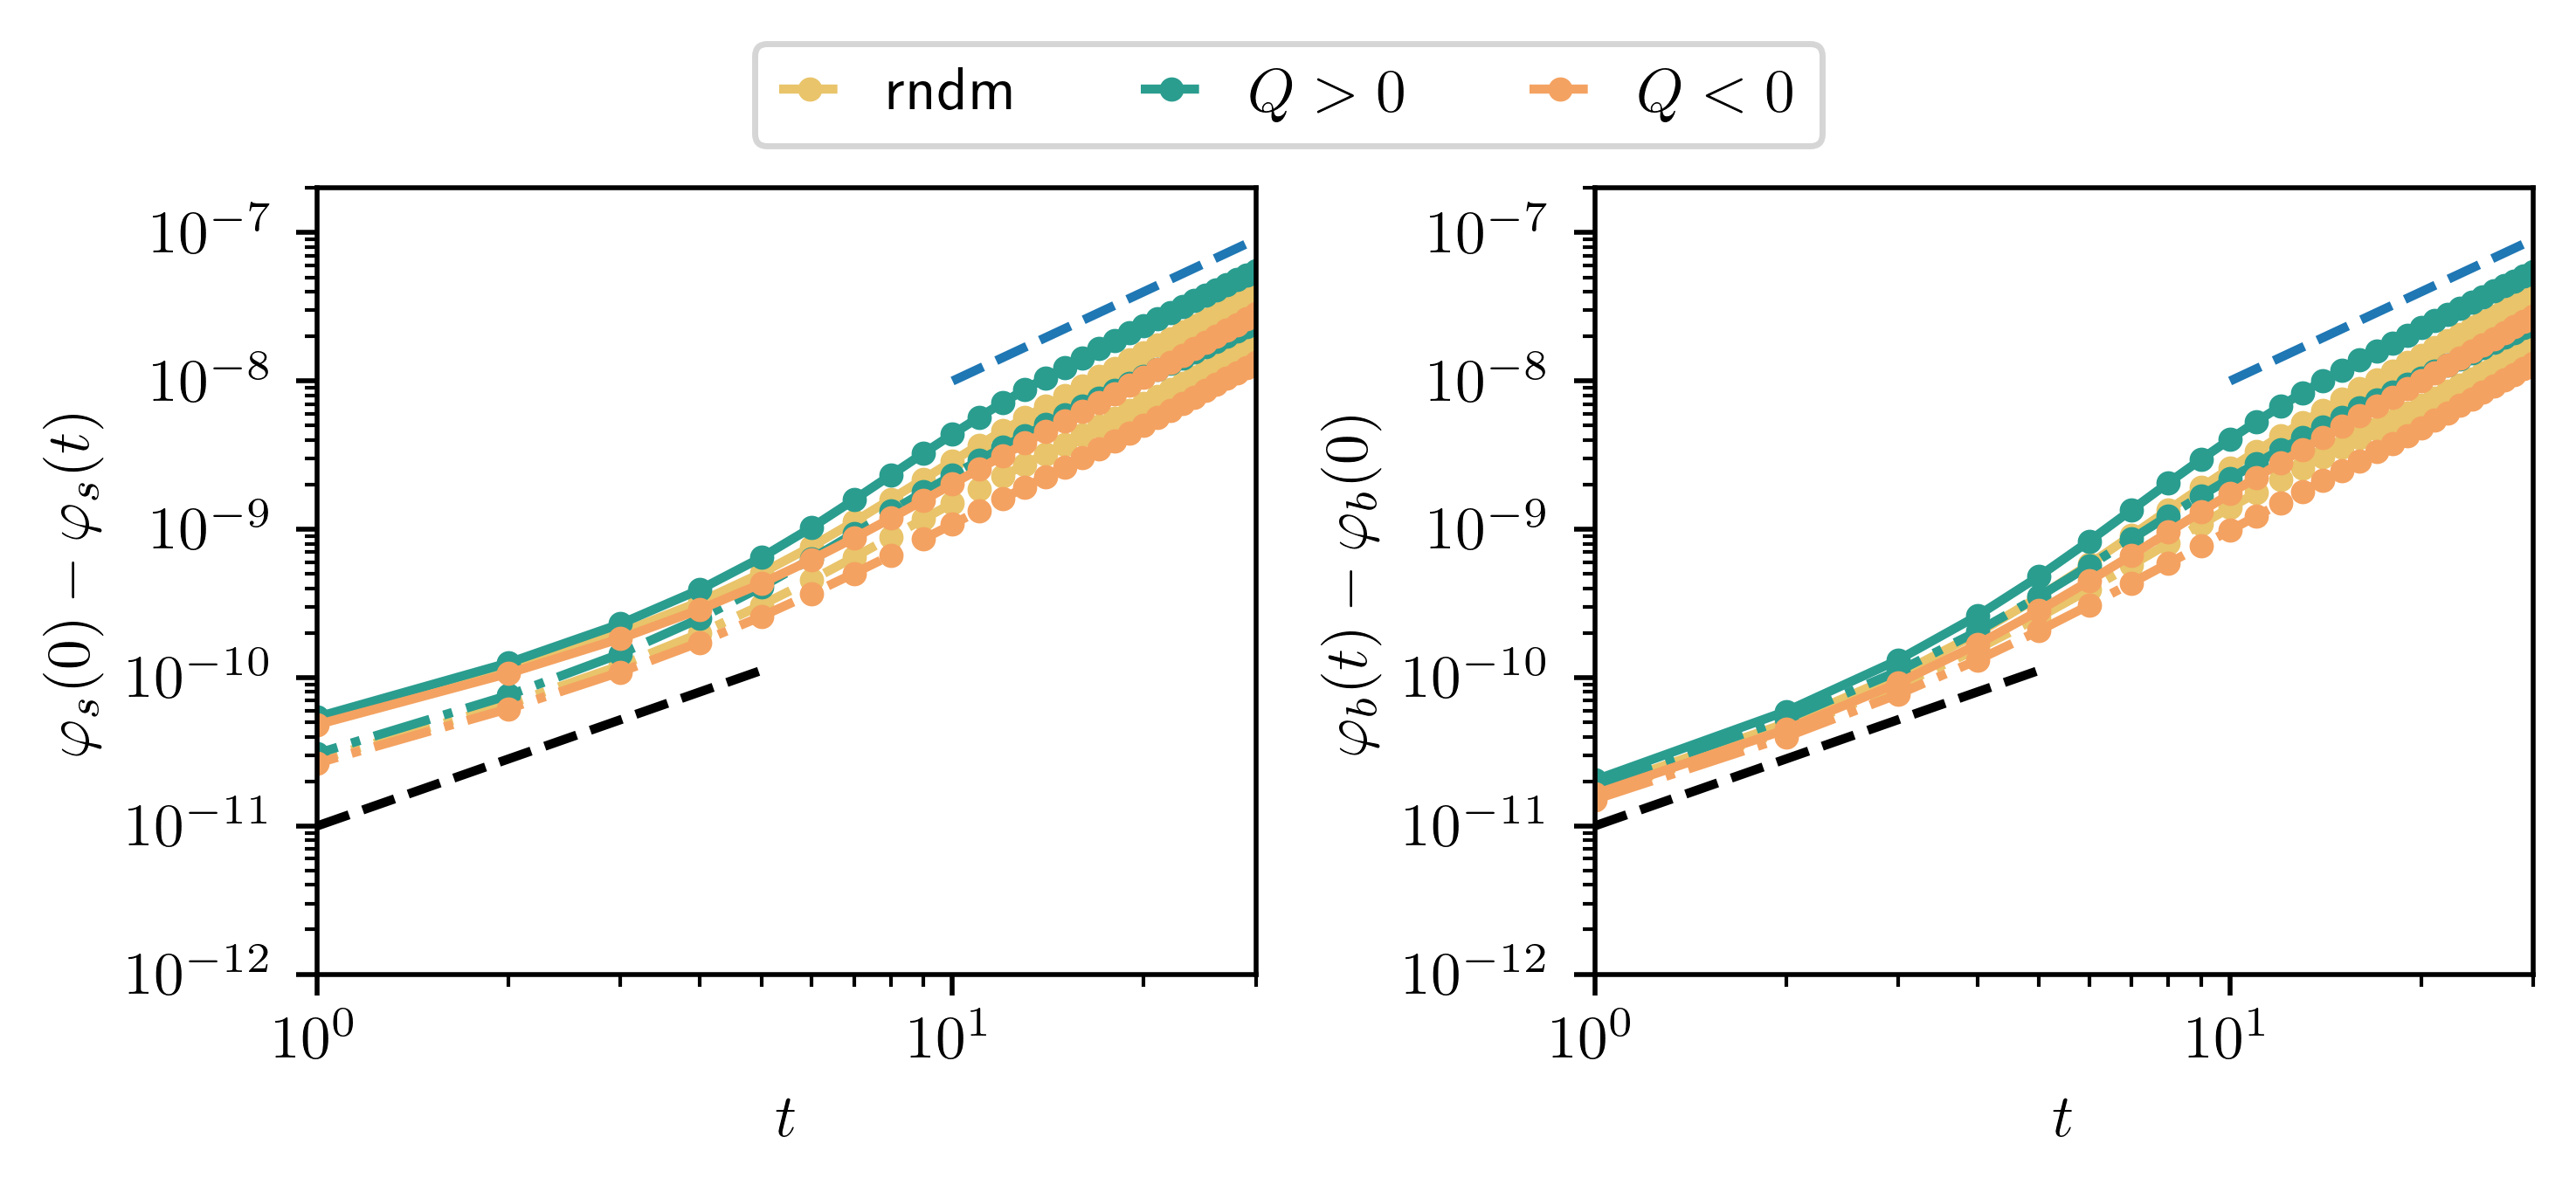
\includegraphics[width=\linewidth]{./figures/polydisperse/smalltimes-2d.png}
% 	\end{center}
% \caption[Early-time scaling of the droplet volume fractions]{Depletion and growth of volume fraction of small droplets (left) and large droplets(right). It shows $t^\frac32$ scaling given by black dashed line at very early times, but takes over as $t^{2}$ given by the blue dashed line immediately after that.}
% \label{lucky-growth-small-times}
% \end{figure}

% However, as one can see in Fig. \ref{lucky-growth-small-times}, both the growth and depletion follow  $t^\frac32$ only at very early times, it very quickly switches to $t^2$ at late times.

% \subsubsection{Late stage growth and depletion}
% In late stage, situation is different. Lucky droplets contain most of the volume fraction with the small droplets are sparsely distributed in the domain. When collisions between the lucky and the small droplets happen, bulk of the volume of the small droplets gets eaten up due to enormous collision cross-section. And, the collision does not significantly increase the size of the lucky droplets. In this case, the depletion of the small droplets $-\dot{M}_s$ is given by
% \begin{align}
% % \label{}
% \begin{split}
%     \dot{M}_s \propto M_s \implies \dot{M}_s \propto e^{-\lambda_s t} \ ,
% \end{split}
% \end{align}
% where $\lambda_s$ is the depletion rate. Similarly, as before, the rate of change of mass of the big droplets is $\dot{M}_s$ and lucky droplets grow as $M_b(t) = M_T - M_s(t) = M_T - M_s^*e^{-\lambda_s(t - t^*)}$. In Fig. \ref{lucky-largetimes-2d}, we show this behavior by plotting the volume fraction of the small droplets, and the growth rate of the large droplets calculated from the local slope of Fig. \ref{lucky-grwth}(right). Both show behavior similar to exponential, but their slopes do not match.
% \begin{figure}
% 	\begin{center}
% 		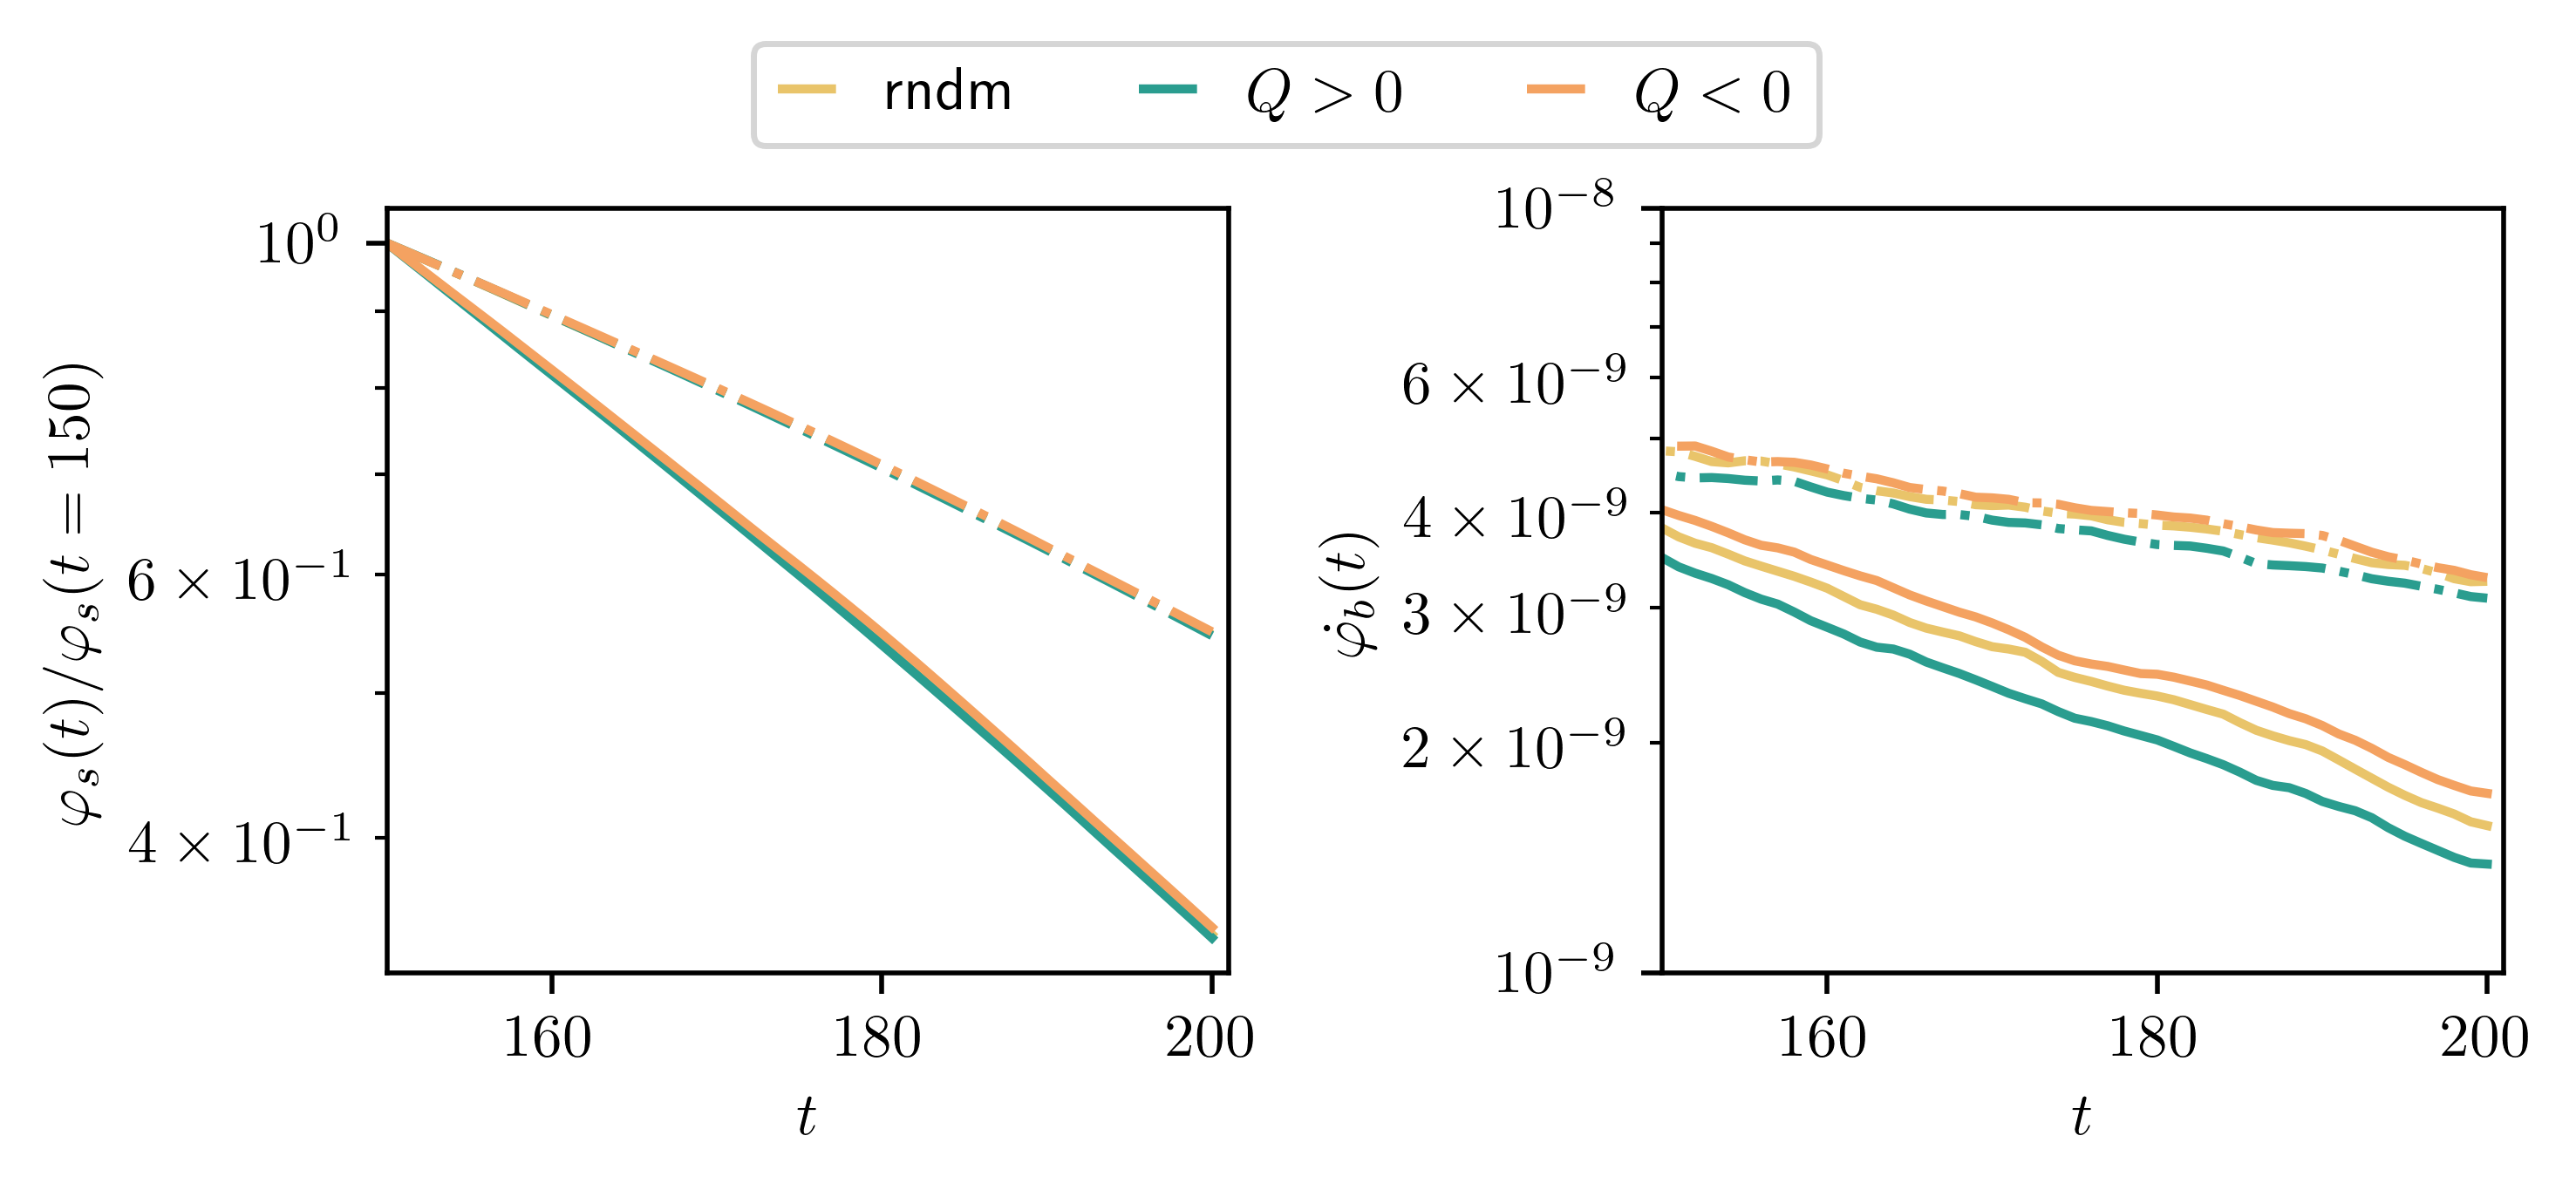
\includegraphics[width=\linewidth]{./figures/polydisperse/largetimes-2d.png}
% 	\end{center}
% \caption[Late-time exponential decay of the droplet volume fractions]{(left) Volume fraction of small droplets at late times. It follows exponential decay. (right) Rate of change of volume fraction of large droplets calculated from local slope. As expected, it also follows exponential decay.}
% \label{lucky-largetimes-2d}
% \end{figure}
% \begin{table}
%     \centering
%     \renewcommand{\arraystretch}{2} % spacing between rows
%     \begin{tabular}{cccc}
%     \hline
%     \textbf{St} & \textbf{Init} & $\lambda_s$ \textbf{ left} & $\lambda_s$ \textbf{ right} \\ \hline
%     0.01 & rndm   & -0.02128 & -0.01720 \\
%     0.02 & rndm   & -0.01203 & -0.00760 \\
%     0.01 & $Q>0$  & -0.02134 & -0.01809 \\
%     0.02 & $Q>0$  & -0.01208 & -0.00770 \\
%     0.01 & $Q<0$  & -0.02101 & -0.01675 \\
%     0.02 & $Q<0$  & -0.01196 & -0.00744 \\ \hline
%     \end{tabular}
%     \caption[Fitted slopes for the late-time volume fractions]{Fitted slopes $\lambda_s$ for the left and right part of Fig. \ref{lucky-largetimes-2d}. They do not match.}
% \end{table}



% Now, although the growth rate for smaller initial $St_b$ are higher, do they produce droplets that cross a certain size threshold faster? The answer is YES! Suprisingly, the drops with larger initial $St_b$ has slower growth due to smaller number of particles, each of those particles gets to eat up a lot of small droplets and grow faster. Figure \ref{lucky-thresh} demonstrates this phenomenon.

% \begin{figure}
% 	\begin{center}
% 		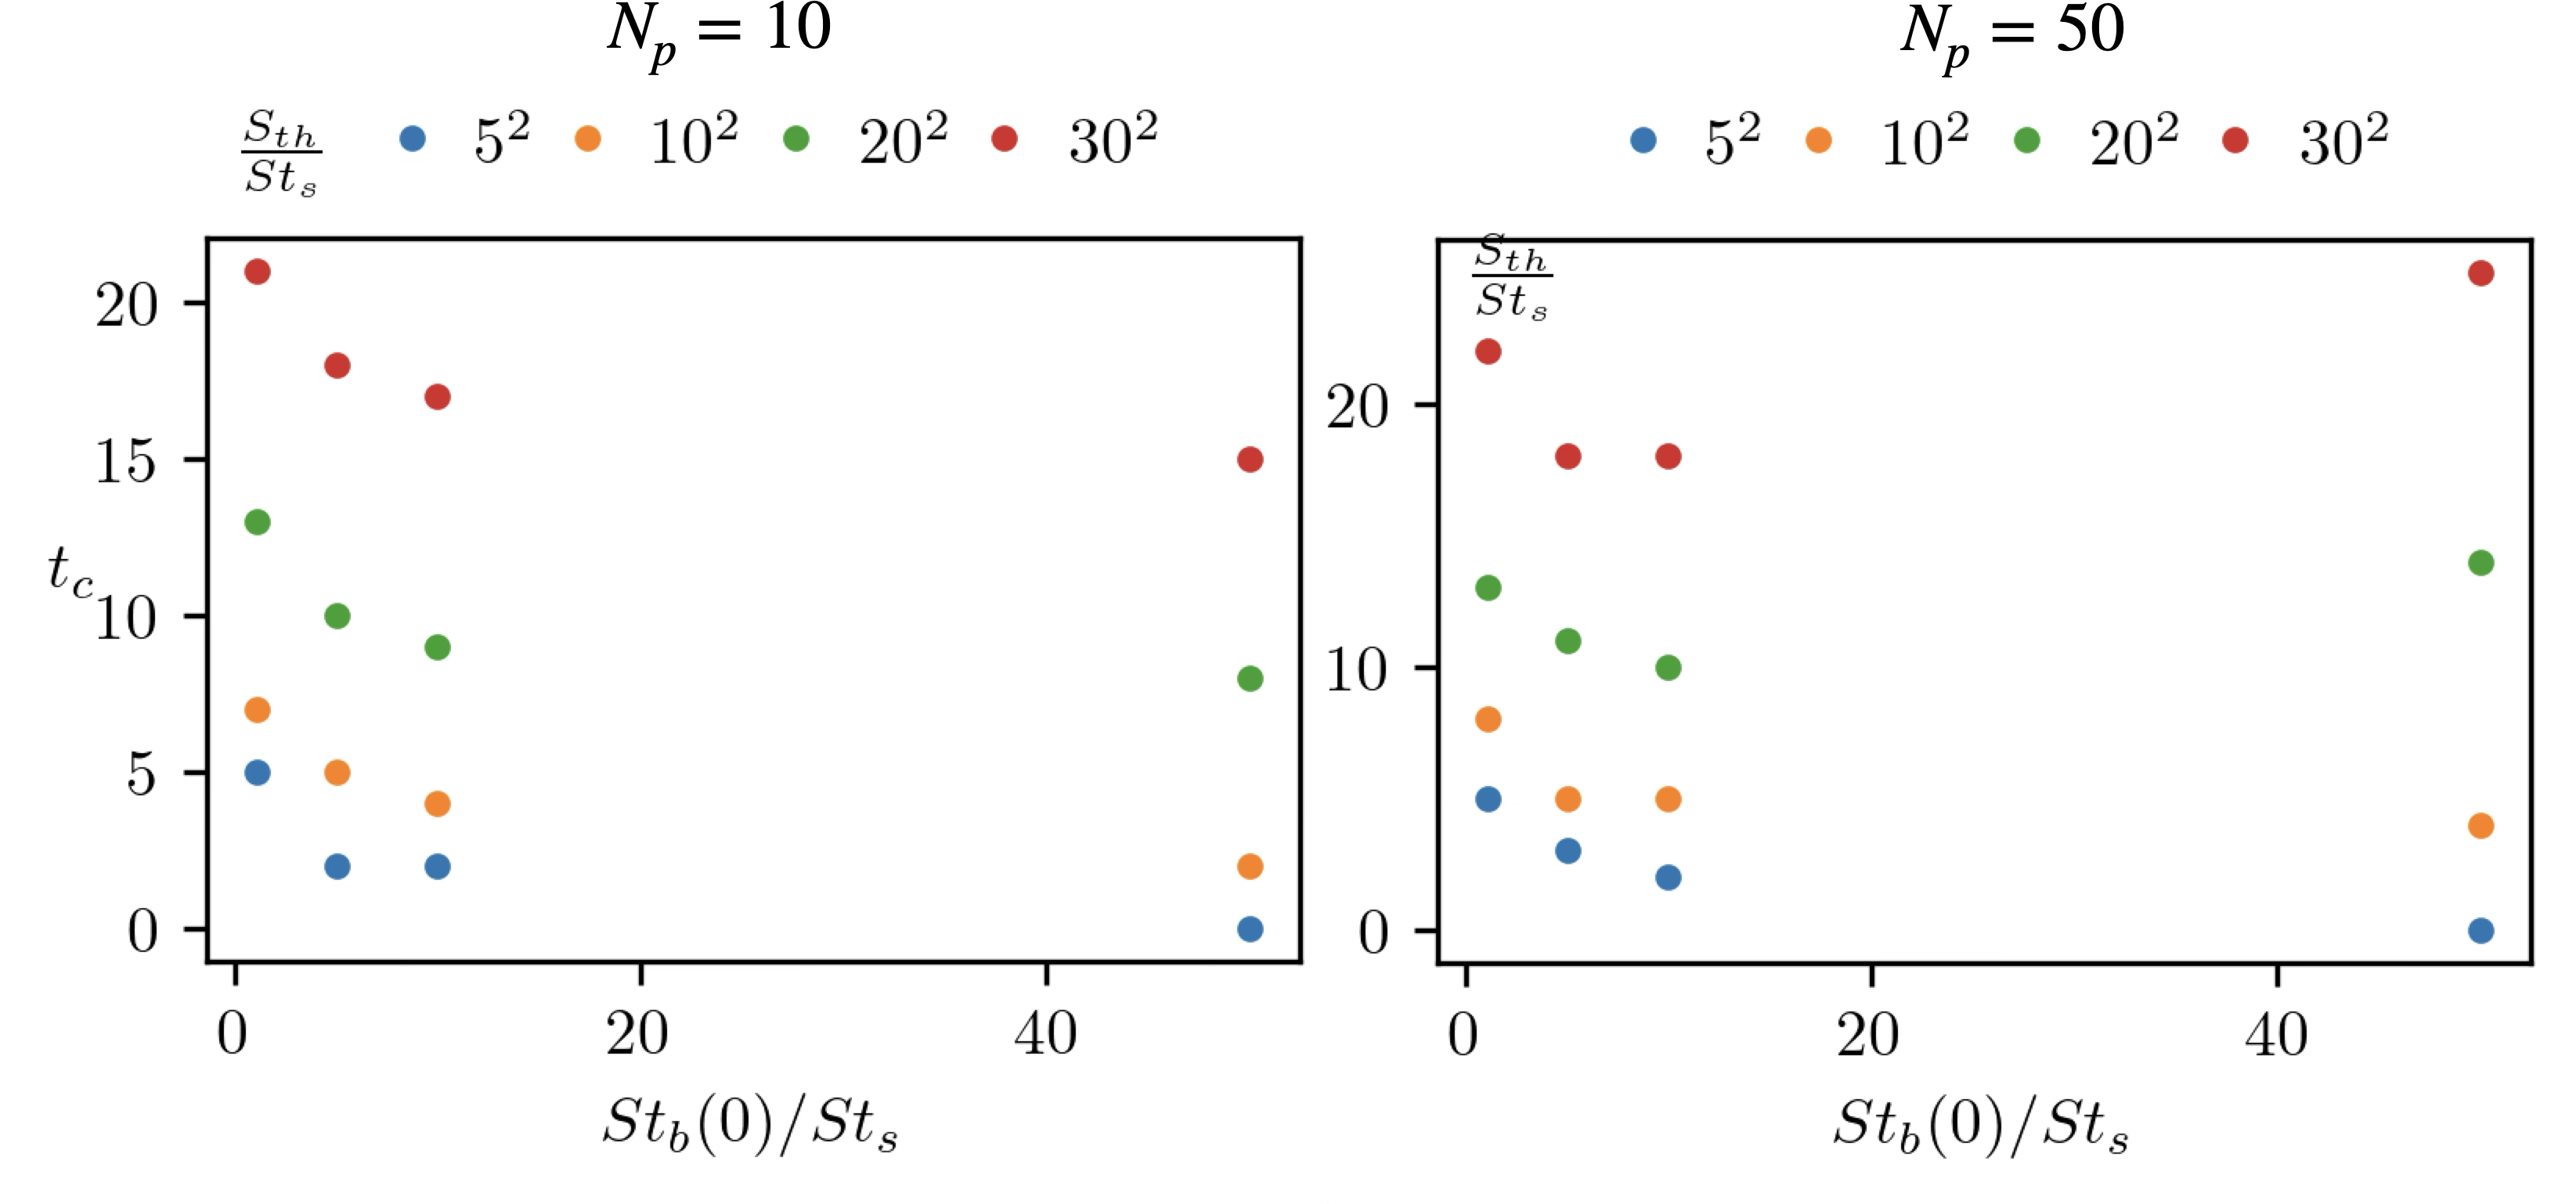
\includegraphics[width=\linewidth]{./figures/polydisperse/threshold-growth.png}
% 	\end{center}
% \caption[Time for big droplets to grow past a threshold]{Time taken for 10 particles (left) and 50 particles (right) to grow beyond a certain threshold for different initial $St_b$s}

% \label{lucky-thresh}
% \end{figure}


% % \begin{figure}
% % 	\begin{center}
% % 		\includegraphics[width=\linewidth]{plots/threshold-growth-50.png}
% % 	\end{center}
% % \caption{Same as Fig. \ref{lucky-thresh} but for 50 particles.}
% % % \label{}
% % \end{figure}
\section{3D results}

\subsection{Growth during Gravitational Settling}
In Section \ref{grav-sett-anltc}, we derived how radius grows with time with the assumption that the lucky particles are always settling in terminal velocity. Here we compare that result with the numerical solution of Eqs. \ref{mass-cont} and \ref{mon-cont} with $\vec{u} = 0$ and $c_s(\vec{x}_b, t) = 7.2 \times 10^{-7}$. We consider two cases of the numerical solution, one where the deceleration term is ignored, and one where it remains. This is done to see when and how the deceleration term affects the growth rate. In Fig. \ref{grav-settl}, we see that the three cases differ only when the particles become very big compared to its initial sizes. The analytical solution predicts an exponentially increasing growth rate. The growth rate in numerical simulation tapers off, and in presence of the deceleration term, the growth rate decreases faster. Still, the growth rate differs in times of around 30 mins, and only for the biggest lucky droplets. Thus, we can work with the solution of Eq. \eqref{grav-settl-sol} when comparing turbulence induced in $3$D growth with gravitational settling growth.
\begin{figure}
\centering
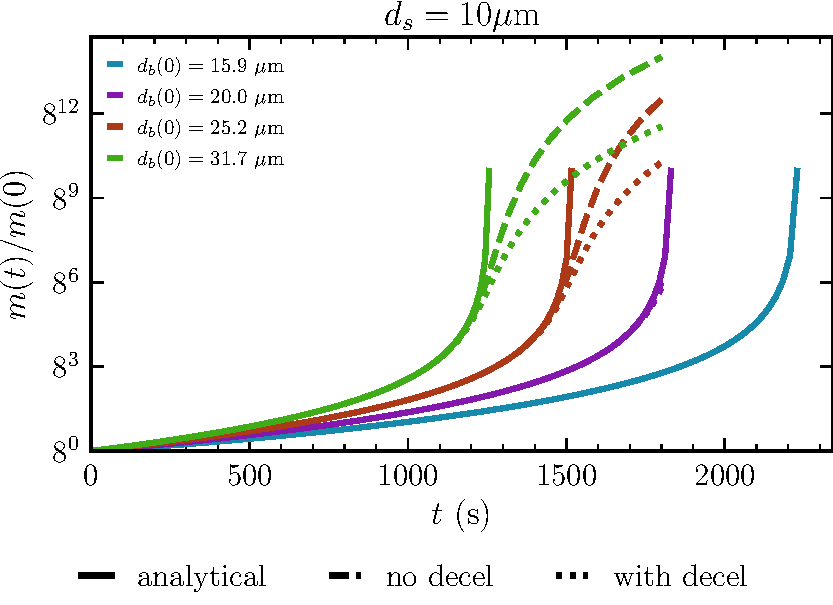
\includegraphics[width = \linewidth]{./figures/polydisperse/gravity_cases.pdf}
\caption{Comparing growth rate with pure gravitational settling. }\label{grav-settl}
\end{figure}

The trend that we see in gravitational settling is different from the $2$D case. The larger lucky drops benefit more while settling, opposite to the conclusion we drew in $2$D. This is because the relative velocity is proportional to the big Stokes number. The total growth rate of each particle scales as $d_b^4$. Now, consider the case where particles of different sizes are different in number such that their net mass is the same.  The number of particles of size $d_b(0)$ $N_p(d_b(0)) \sim 1/d_b^3(0)$, and if the relative velocity between the lucky and the tiny particles scale as $d_b(0)$ initially, the total growth rate scales as $d_s$, making larger particles accumulate more small droplets with time. 
\subsection{Turbulence assisted growth}
We now turn to $3$D turbulence where the lucky droplets grow in presence of the flow. Fig. \ref{turb-grav} shows that turbulence hardly makes any change in droplet growth compared to the gravitational settling. In fact, for some lucky droplets turbulence decreases their growth, which is quite interesting. This little change from turbulence is disheartening but expected. Given that the Froude number $Fr$ is so small in table \ref{lucky-cloud-vals}, turbulent accelerations on the particles  should be very weak compared to gravity forces. This confirms an important point. Turbulence with the mean dissipation rate observed in cannot significantly control droplet growth. It can only contribute in patches with dissipation significantly higher than the mean dissipation rate.  
\begin{figure}
\centering
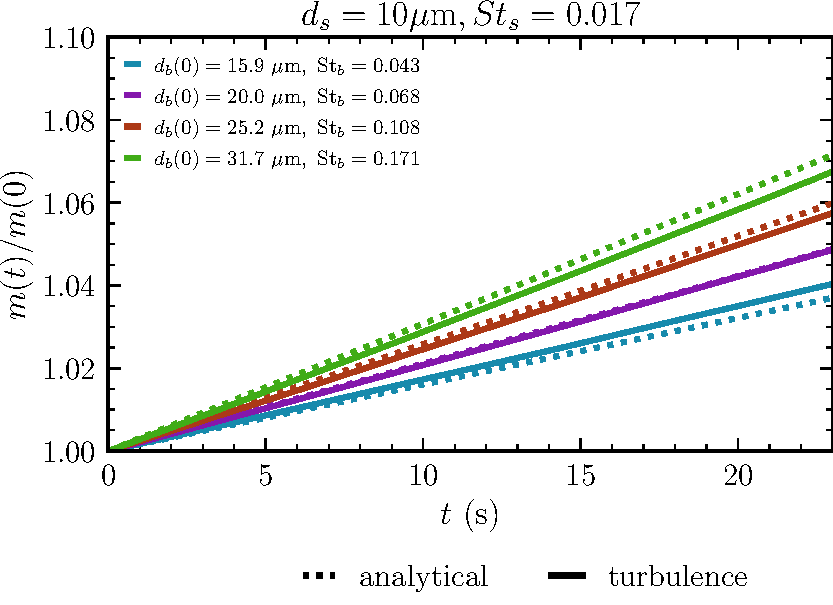
\includegraphics[width = \linewidth]{./chapters/figures/polydisperse/turb-gravity-withg.pdf}
\caption{Comparing turbulence assisted droplet growth in presence of gravity and growth during gravitational settling for different Stokes number(sizes). The lucky droplets started in random locations of the flow with tiny droplets having Stokes $0.017$, the Kolmogorov length and timescales are matched with case with $\epsilon = 10^{-2}\text{ m.s}^{-1}$ in table \ref{lucky-cloud-vals}.}
\label{turb-grav}
\end{figure}

When we compare growths in presence and absence of gravity, in Fig. \ref{turb-g-no-g}, we find that turbulent contribution is miniscule at such Stokes and Froude numbers. This is even more disheartening because we want gravitational effects to dominate at larger sizes. But it seems to win, even at such small sizes. An interesting trend to notes is that the bigger lucky droplets grows faster even in absence of gravity. Thus, the hand-waving argument given in the last section still holds here. 
\begin{figure}
\centering
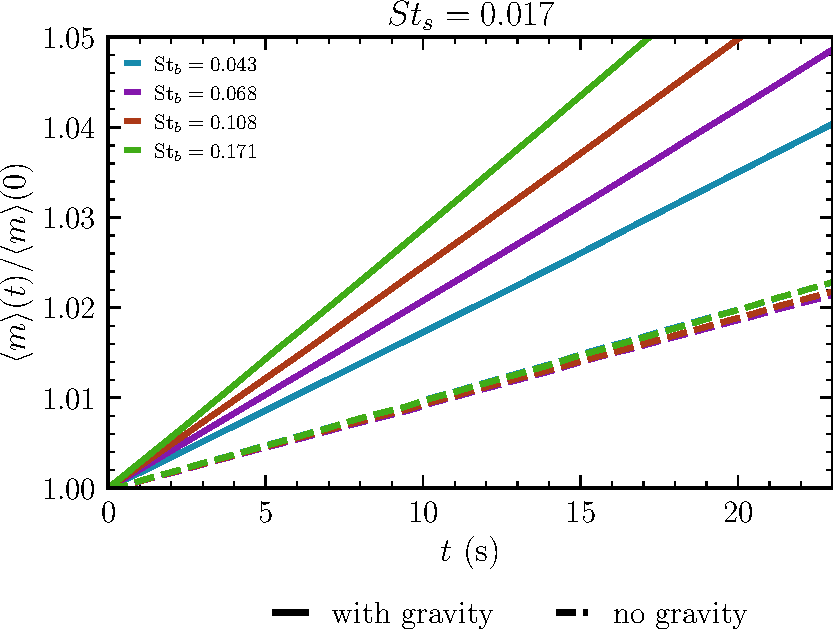
\includegraphics[width = \linewidth]{./chapters/figures/polydisperse/turb-g-no-g.pdf}
\caption{Comparing turbulence assisted droplet growth in presence and absence of gravity. Growth without gravity is negligible compared to growth with gravity. The lucky droplets started in random locations of the flow with tiny droplets having Stokes $0.017$, the Kolmogorov length and timescales are matched with case with $\epsilon = 10^{-2}\text{ m.s}^{-1}$ in table \ref{lucky-cloud-vals}.}
\label{turb-g-no-g}
\end{figure}

When we look at the droplet growth rate across different initial conditions in Fig. \ref{turb-init}, the answer is also anti-climactic. We cannot find any significant differences. Our guess for this is the following. In $2$D turbulence, strong gradients like coherent vortices and the strain regions between them, are stable. However, in $3$D turbulence  high gradient regions in $3$D have a very short lifetime. Therefore, their impact is not felt during the droplet growth of the particles starting out in high gradient regions.

\begin{figure}
    \centering
    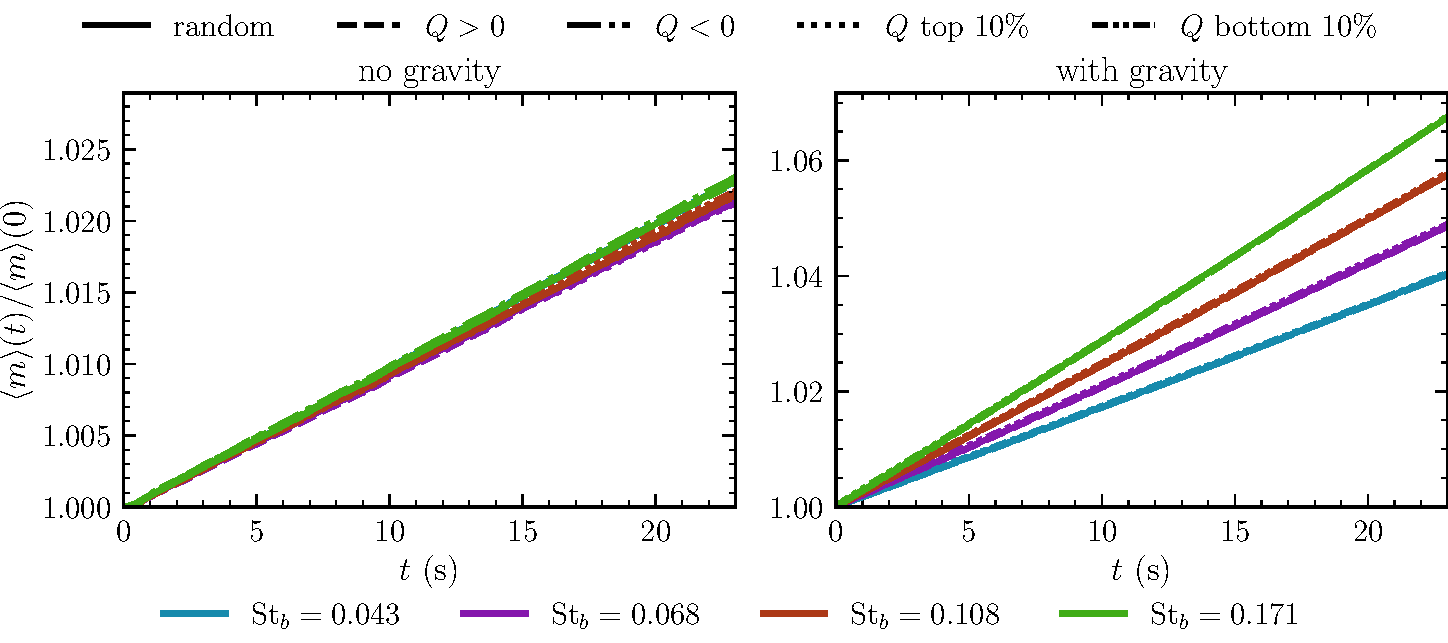
\includegraphics[width = \linewidth]{./chapters/figures/polydisperse/turb-init.pdf}
    \caption{Comparing turbulence assisted droplet growth in presence and absence of gravity with lucky droplets starting from different initial conditions. The different initial conditions make no difference in early time droplet growth. The tiny droplets have Stokes $0.017$, the Kolmogorov length and timescales are matched with case with $\epsilon = 10^{-2}\text{ m.s}^{-1}$ in table \ref{lucky-cloud-vals}.}
    \label{turb-init}
\end{figure}
% \begin{figure}
% 	\begin{center}
% 		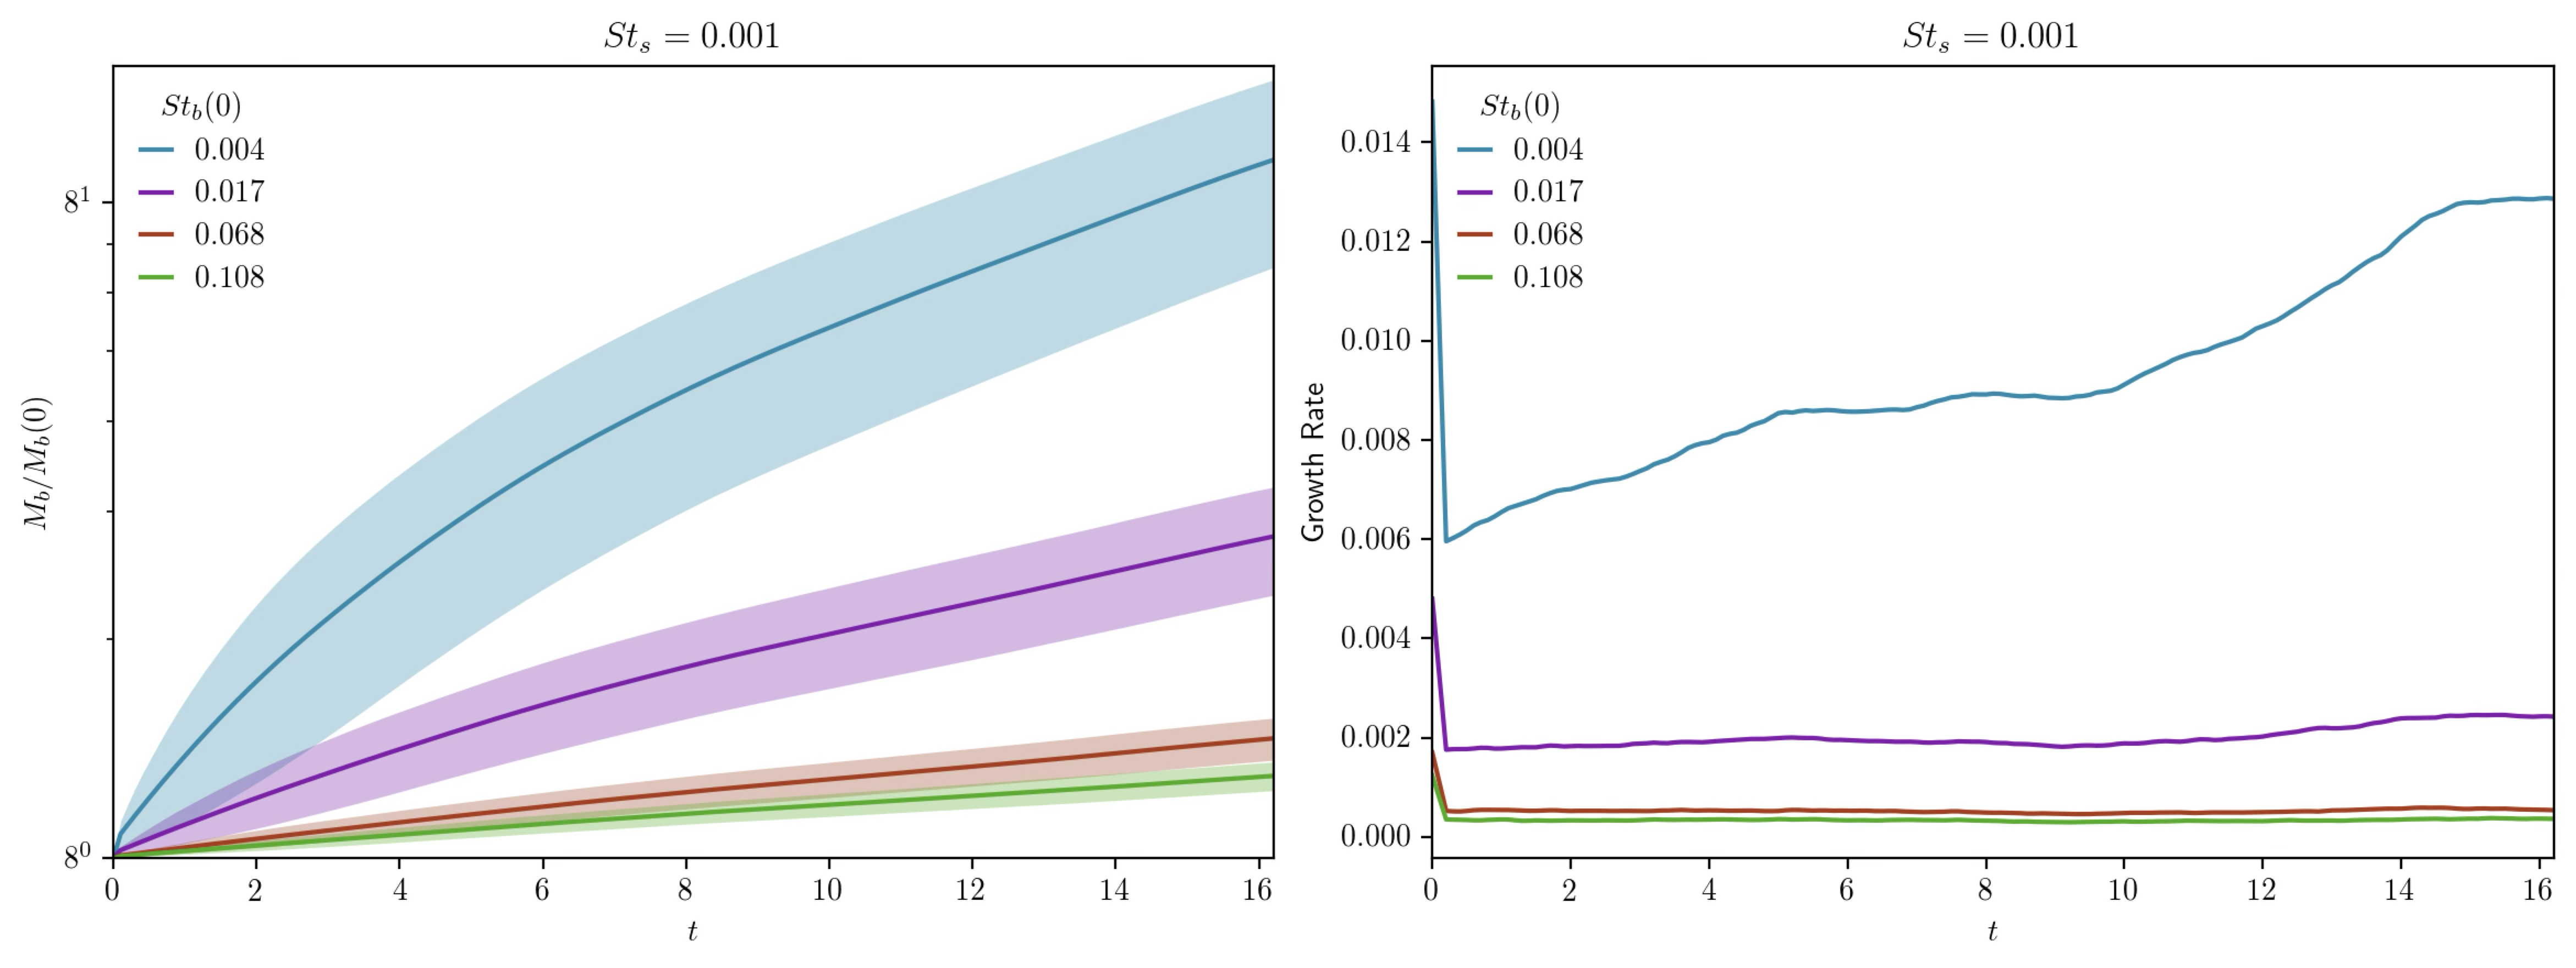
\includegraphics[width=\linewidth]{./figures/polydisperse/3d-grwth.png}
% 	\end{center}
% \caption[Growth in volume fraction of lucky droplets in three dimensions]{Growth in volume fraction of lucky droplets in $3$D}
% \label{lucky-3d-grwth}
% \end{figure}
% According to back at table \ref{lucky-cloud-vals}, we chose $St_s = 0.001$ with an initial liquid water content $c_s(0) = 7.2\times 10^{-7}$. This means that there are $10^{11}$ $2.7\,\mu\mbox{m}$(diameter) particles in a cloud of $1\mbox{m}^3$ with mean dissipation rate $\epsilon = 10^{-2} \mbox{m}^2\cdot\mbox{sec}^{-3}$. After evolving the small particles for significant enough time, put 1 in a million lucky droplets of size $10\,\mu\mbox{m}$. From table \ref{lucky-cloud-vals}, we see that their initial volume fraction must be $c_b(0) = 5\times 10^{-13}$. Given mass of each particle $m_p$ is related to the Stokes number as
% \begin{align}
% % \label{}
% \begin{split}
%     m= 36\pi\rho\left(\frac{\nu\tau_\eta}{2\rho}\right)^\frac32\times St^\frac32,
% \end{split}
% \end{align}
% the number of lucky drops $N_b$ is constrained by the net liquid water content per unit volume, i.e.,
% \begin{align}
% % \label{}
% \begin{split}
%     \frac{N_b\times m_b(0)}{\left(2\pi\times \frac{\eta}{\eta_s}\right)^3 } = \rho c_b(0) \implies N_b \sim 8,
% \end{split}
% \end{align}
% with the parameters described above and where $\eta_s = \mathrm{m}/k_{\mathrm{m}} = 3 \mathrm{m} /(N_g\sqrt2)$ is Kolmogorov length in the simulation units, $k_{\mathrm{m}}$ is the maximum de-aliased wavenumber, $\mathrm{m}$ is given by our choice, and $N_g$ is the resolution of the simulation. This is an abysmally small number. Rather we seed 1 lucky droplet for every 1000 small droplets. This makes the $N_b  \sim 8000 \sim 8192$. Keeping the initial liquid water content of the lucky droplets constant, we change the Stokes number of the lucky droplets. This lets us investigate whether luckier droplets get luckier. The initial lucky drops Stokes number we use are $St_b(0) = [2\times 10^{-3}, 4 \times 10^{-3}   , 0.017     , 0.068     , 0.11   ]$.


% At a first glance of Fig. \ref{lucky-3d-grwth}, the results for $2$D still holds for $3$D. But the growth is very minimal. This is expected in $3$D as the collision cross-section is smaller, owing to fewer collisions. This means that one has to evolve the system for longer times which is quite difficult in $3$D. In fact, while evolving different cases of initial lucky droplets, the bottleneck becomes evolving the field equations of $n$. Each class of lucky droplets require a separate number density field because of the mutual couplings between the small and big particles. The evolution of number density field incurs more Fast-Fourier transforms which are time-consuming.

% We can make significant progress if we statistically model the small particles. That is not always easy. Preferential clustering of inertial particles introduce spatial correlations in their number density. This is different from tracers that randomly distribute themselves in an incompressible homogenous isotropic flow, making their number density follow a Poisson distribution. Large Stokes particles also follow this as they are almost ballistic and randomly run around in the flow. Tiny Stokes particles following Eq. \eqref{lucky-3Deqns} are also tracerlike, with perturbations proportional to the flow acceleration. And, if the maximum flow acceleration is much smaller than the Stokes number, the small Stokes particles \emph{almost} distribute themselves like tracer.
% \begin{figure}
% 	\begin{center}
% 		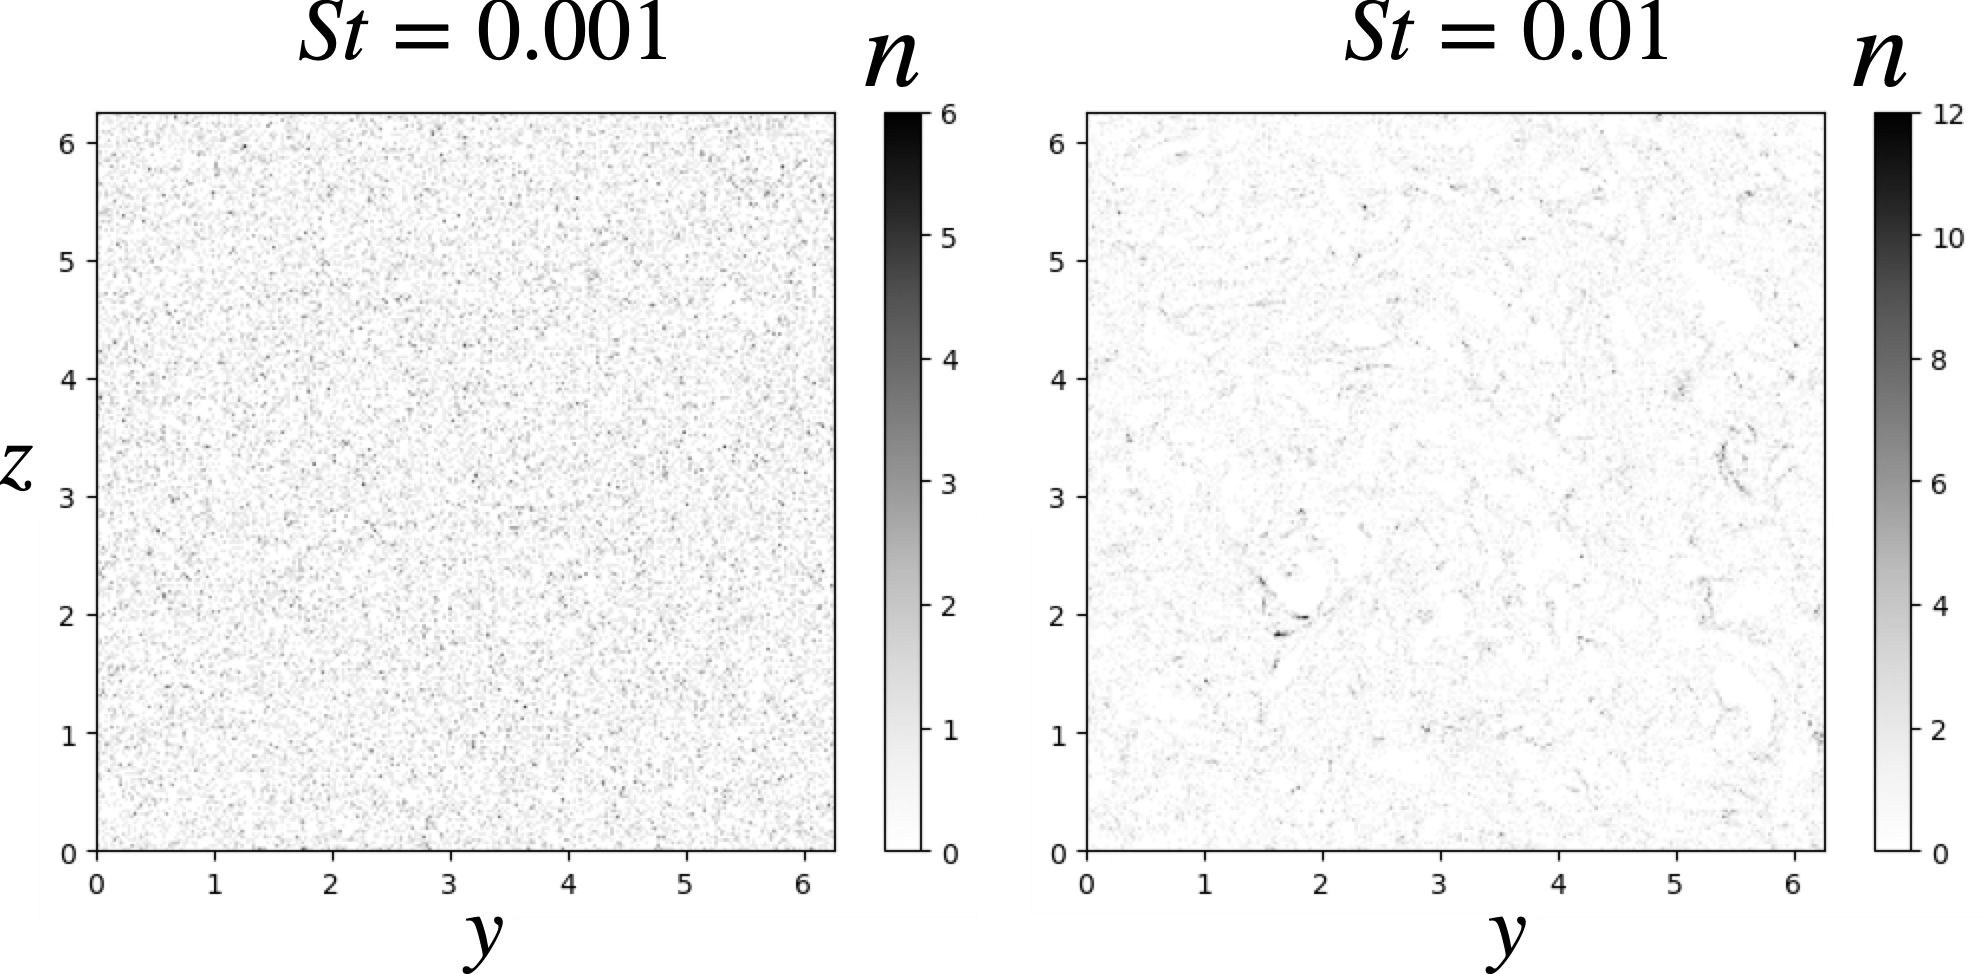
\includegraphics[width=\linewidth]{./figures/polydisperse/dist-nbin-256.png}
% 	\end{center}
% \caption[Binned number density of Lagrangian tiny droplets]{Binned number density if Lagrangian tiny particles following Eq. \eqref{lucky-3Deqns}. A total of $4\times 128^3$ particles are binned in $256^3$ grid.}
% \label{lucky-nbin-dist-256}
% \end{figure}

% This is evident in Fig. \ref{lucky-nbin-dist-256} where the number density of $4\times 128^3$ particles binned in $256^3$ grid shows a spotty pattern for $St = 0.001$ but some correlation in $St = 0.01$. Increasing the grid size in Fig. \ref{lucky-nbin-dist-128} further illustrates the correlation of $St= 0.01$ particles. The structure of the $St = 0.01$ particles is well correlated with the local flow gradients, seen in Fig. \ref{lucky-grad-corr}. The spottiness of $St = 0.001$ fields hints at a spatially uncorrelated structure, and therefore a Poisson distribution. Indeed, it can be well approximated by Poisson distribution as Fig. \ref{lucky-poisson-check}. The mean of the Poisson distribution is the mean number of particles in the specified box size.




% \begin{figure}
% 	\begin{center}
% 		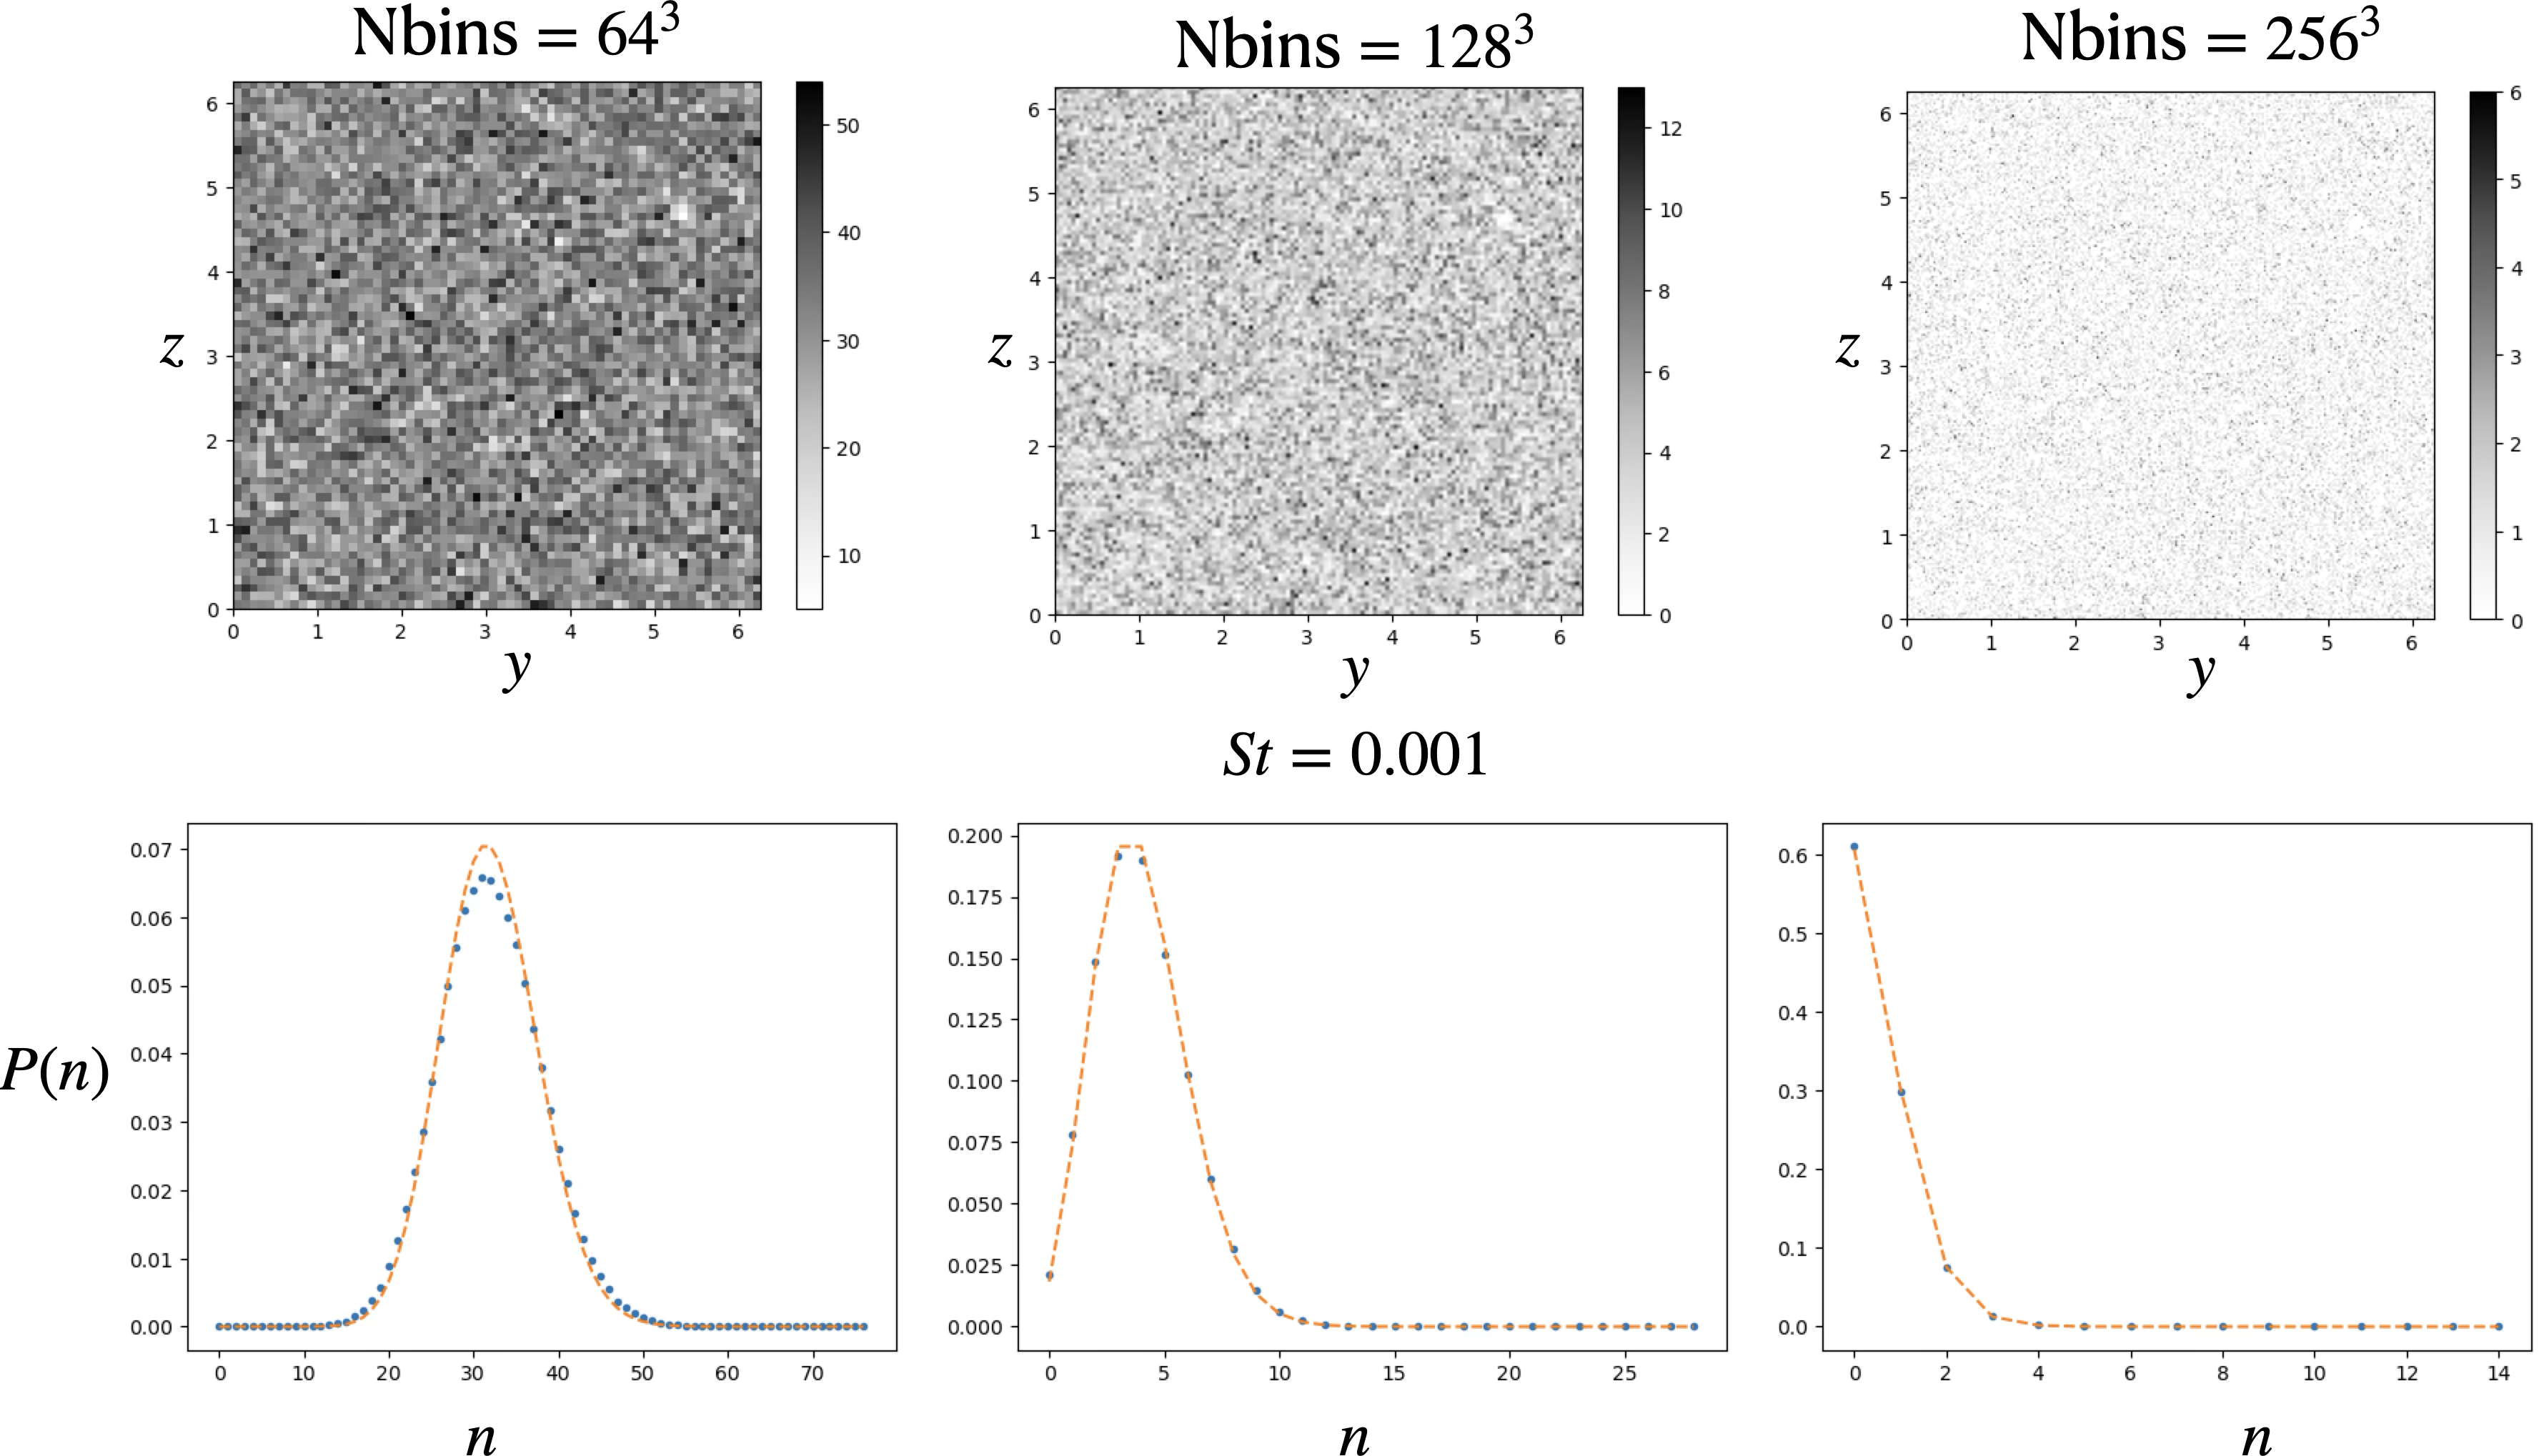
\includegraphics[width=\linewidth]{./figures/polydisperse/poisson-check.png}
% 	\end{center}
% \caption[Binned number density compared with a Poisson distribution]{Structure of binned number density and the Poisson distribution across different number of bins. The number density (blue) deviates from the Poisson distribution (orange) at large scales due to deviation from tracer trajectories. }
% \label{lucky-poisson-check}
% \end{figure}

% Note that at larger scales, the number density does not obey a Poisson distribution. This is because the particles are not exactly tracer and the fluid acceleration does have some large scale correlation effects. But at the smaller scale, Poisson distribution assumption is a good one. Note that this result only follows in $3$D where large fluid accelerations are not long-lived, in $2$D, persistence of large strong vortices make the number density of tiny droplets spatially well correlated.

% This insight allows us to modify Eq. \eqref{lucky-3Deqns}. We do not evolve the number density of the small particles anymore, rather we draw the number of particles each lucky droplet encounters in a given $\Delta t$ from a Poisson distribution. We still have to evolve the $\vec{v}_s$ equation, and interpolate at the location of the lucky droplets. The result with this is significantly different from the \begin{figure}
% 	\begin{center}
% 		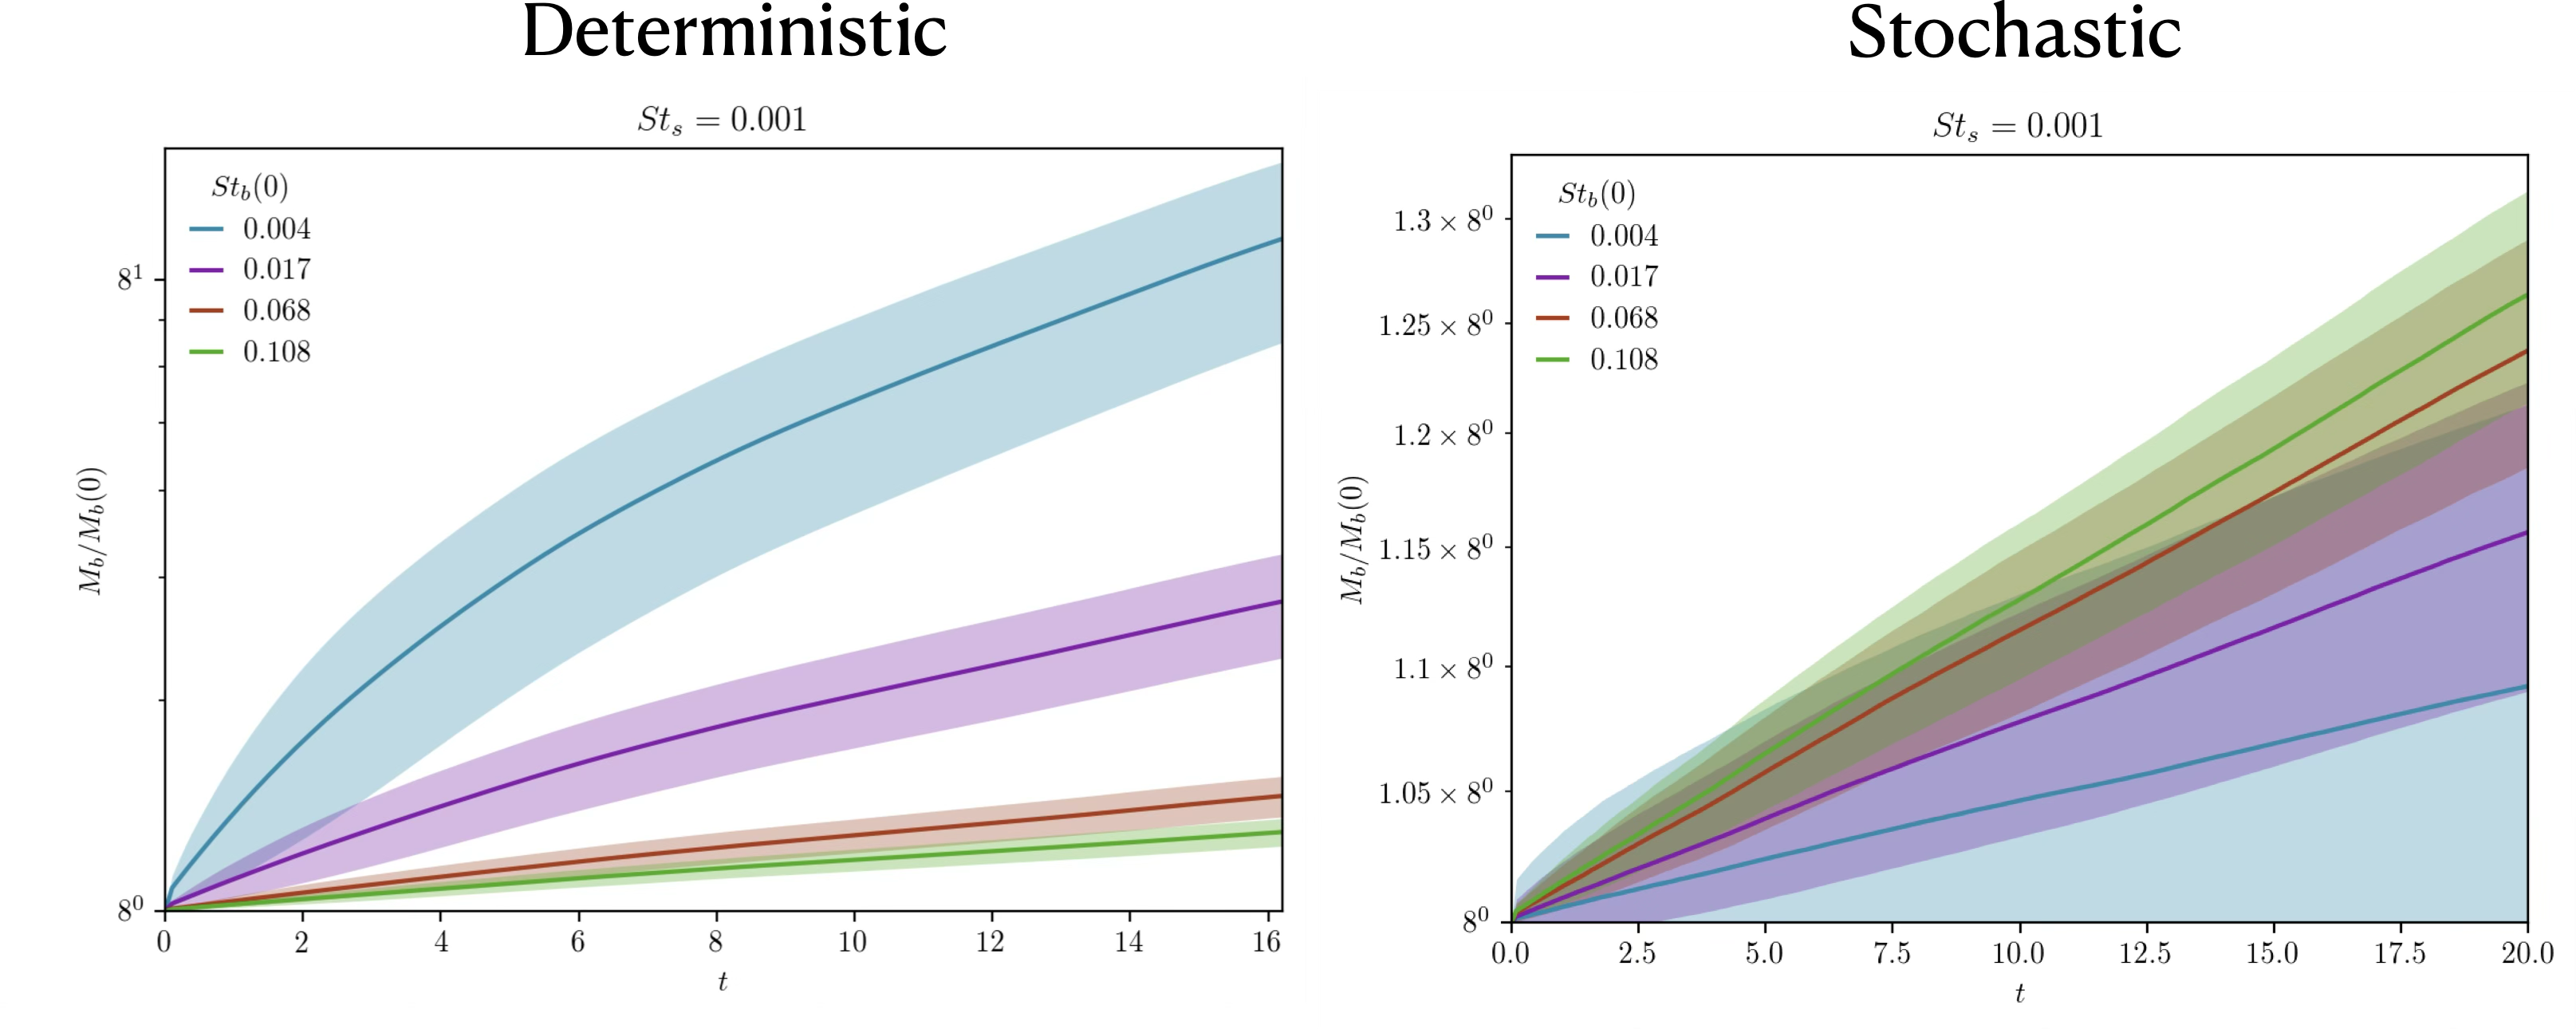
\includegraphics[width=\linewidth]{./figures/polydisperse/det-v-stoch.png}
% 	\end{center}
% \caption[Growth rate from deterministic and stochastic collisions]{Growth Rate of deterministic v stochastic simulations.}
% % \label{}
% \end{figure}

% \begin{figure}
% 	\begin{center}
% 		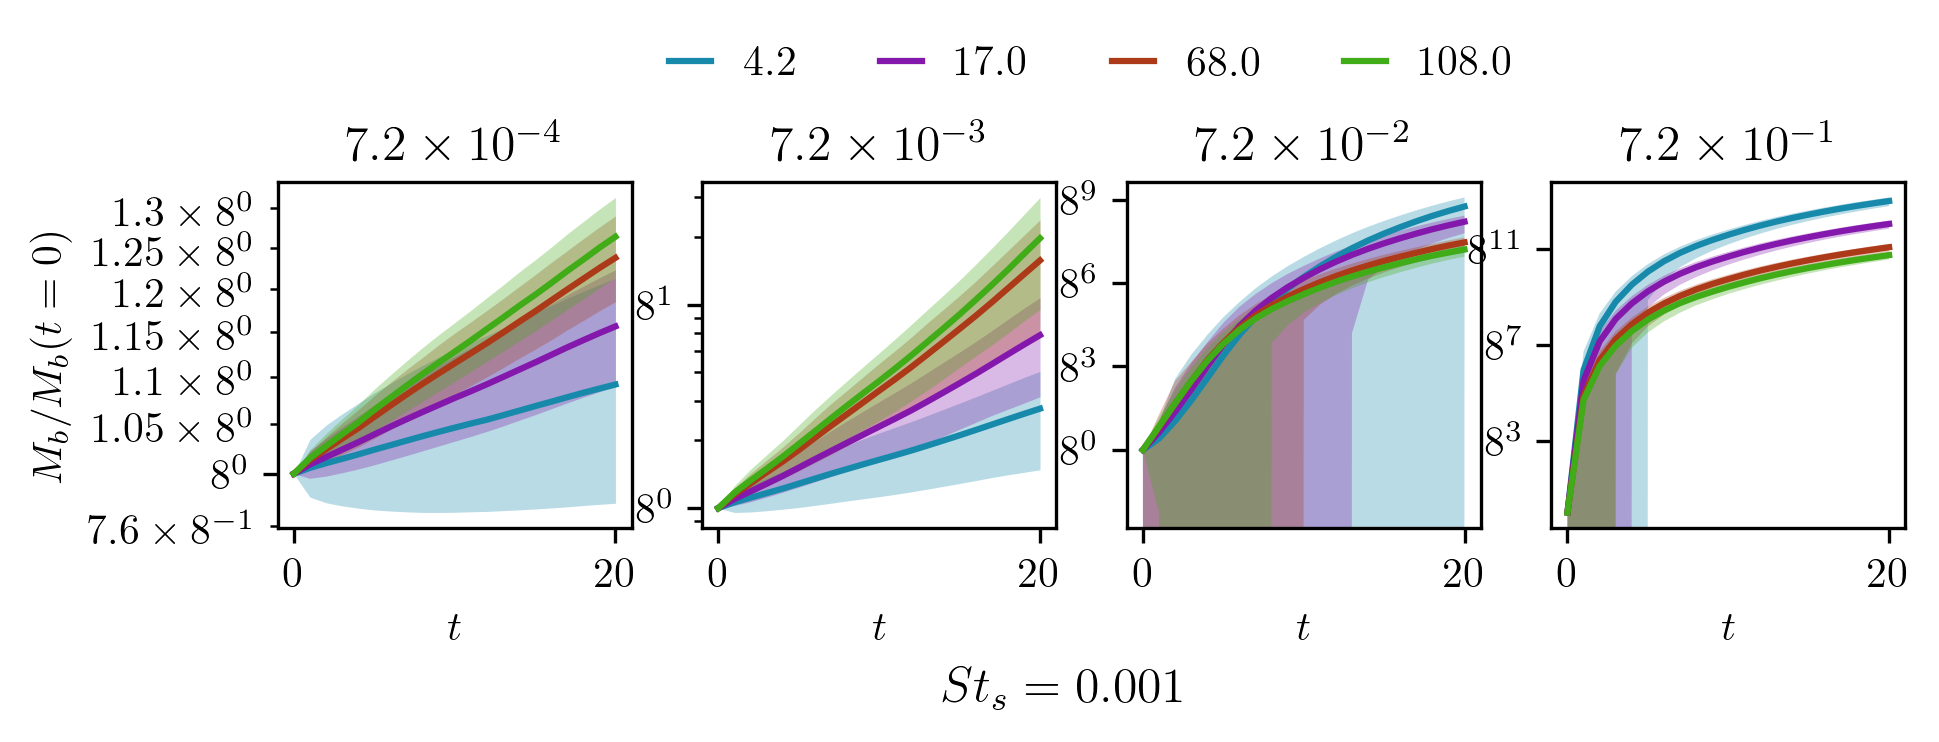
\includegraphics[width=\linewidth]{./figures/polydisperse/stoch-v-m.png}
% 	\end{center}
% \caption[Growth rate for different small-droplet number densities]{Comparison of growth rate after varying small particle number density.}
% % \label{}
% \end{figure}


% \begin{figure}
% 	\begin{center}
% 		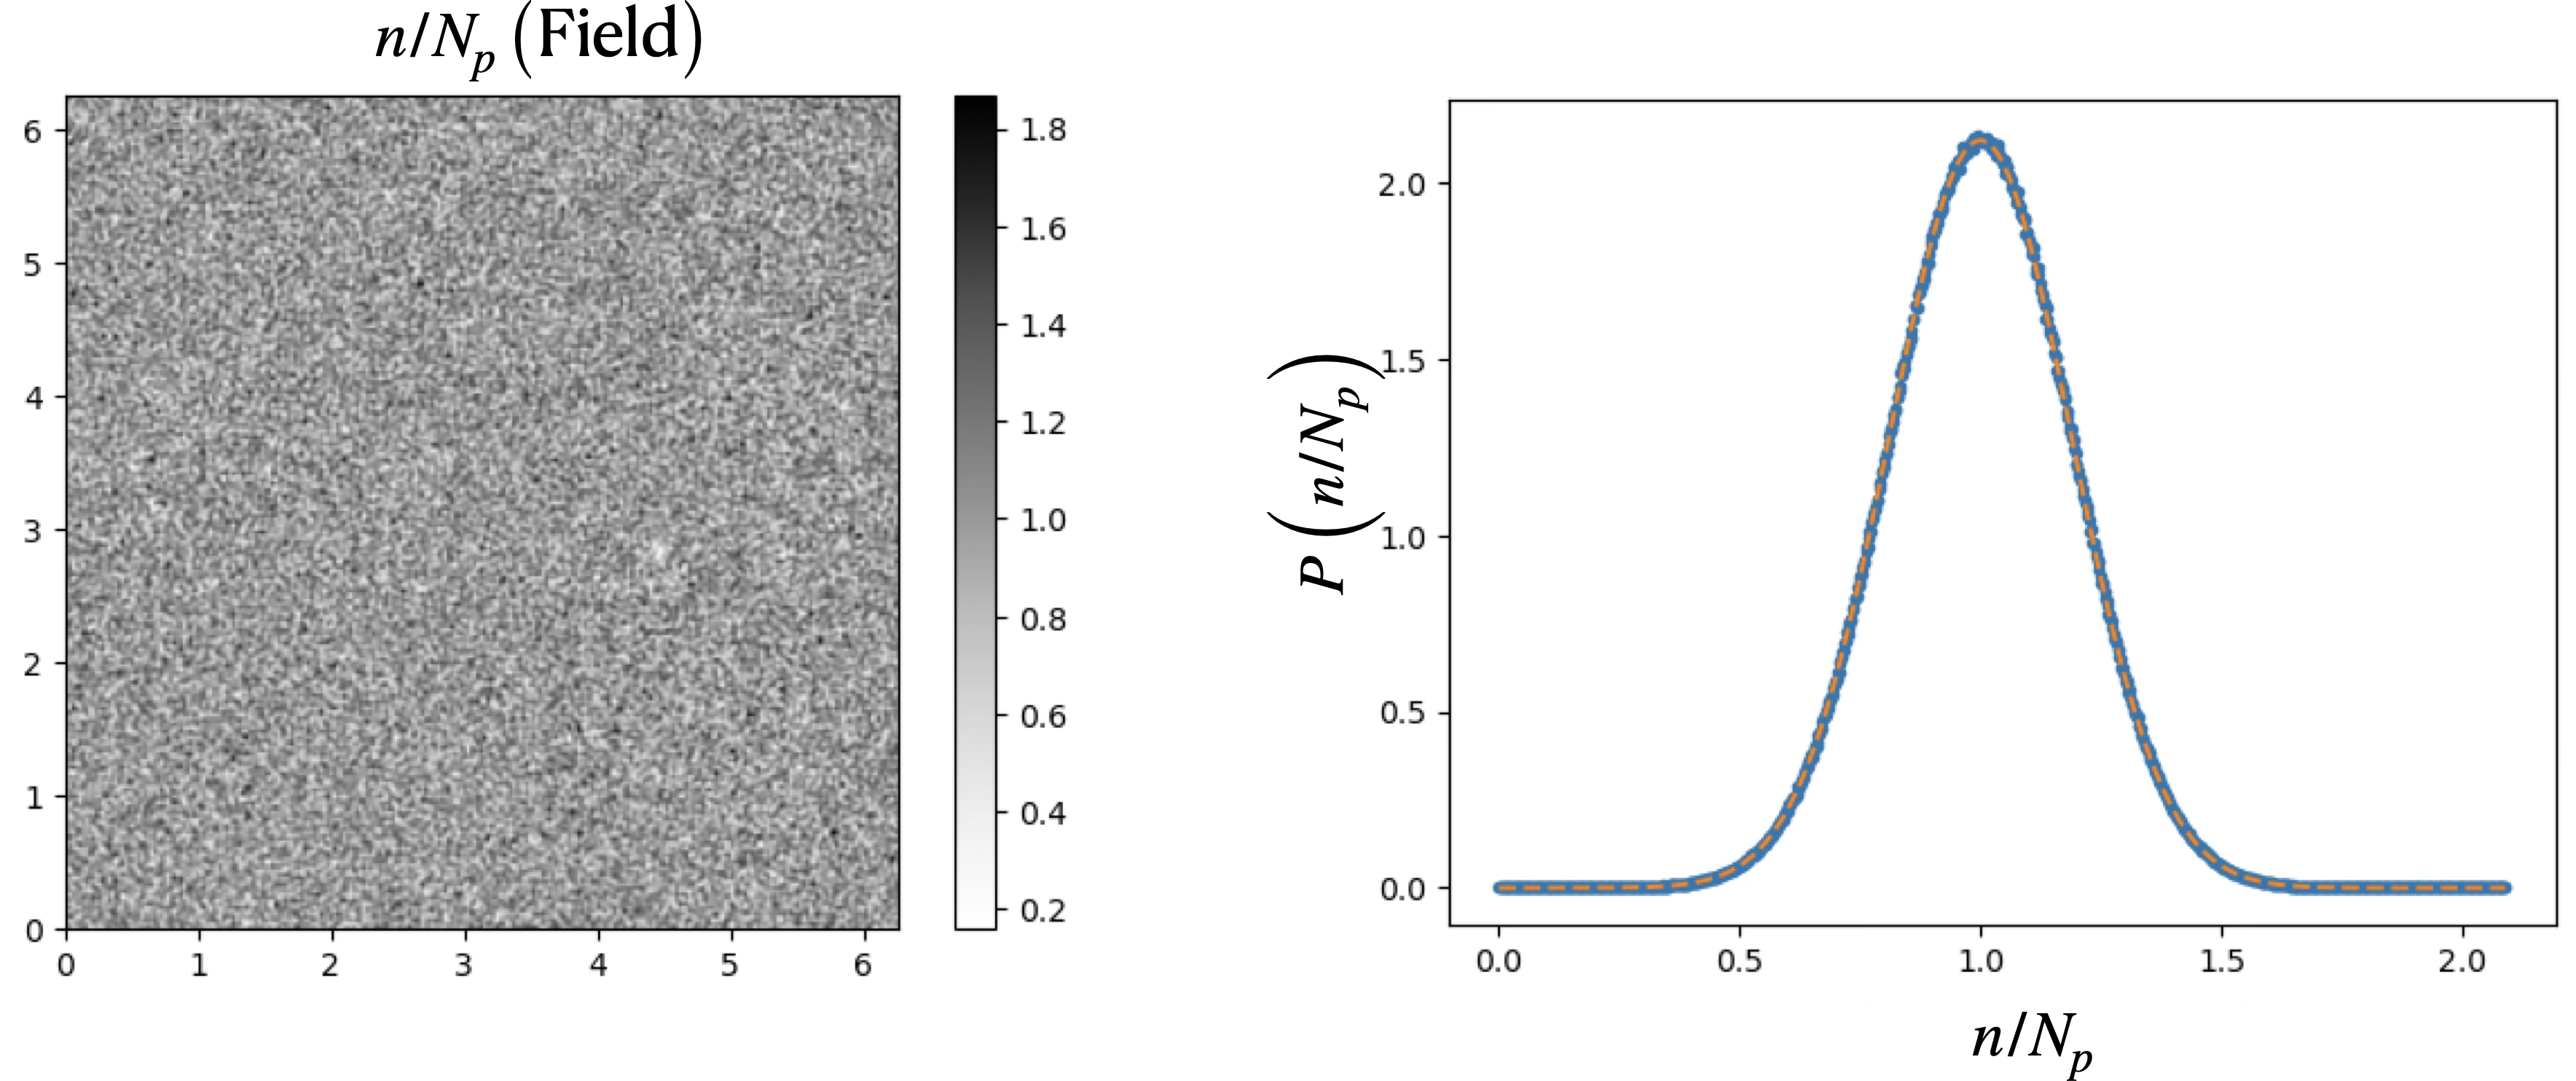
\includegraphics[width=\linewidth]{./figures/polydisperse/nfield-dits.png}
% 	\end{center}
% \caption[Number density field from the continuum model and its distribution]{Snapshot of the number density field evolved from continuum models (left). Its distribution (right) follows a perfect Gaussian with unit mean and standard deviation obtained from the data. }
% \label{}
% \end{figure}



\end{document}
